\chapter{集合}
\section{元素与集合}
\subsection{集合的概念}
虽然集合是一个原始的概念, 但对一个具体的集合而言, 很多情况下我们还是可以采用列举法或描述法给出它的一个准确而清晰的表示.

用描述法表示一个集合基于下面的概括原则:

\textbf{概括原则}\quad 对任给的一个性质 $P$, 存在一个集合 $S$, 它的元素恰好是具有性质 $P$ 的所有对象, 即
$$
	S=\{x \mid P(x)\}
$$

其中 $P(x)$ 表示 “ $x$ 具有性质 $P "$.

由此,我们知道集合的元素是完全确定的, 同时它的元素之间具有互异性和无序性.

集合的元素个数为有限数的集合称为有限集, 元素个数为无限数的集合称为无限集. 如果有限集 $A$ 的元素个数为 $n$, 则称 $A$ 为 $n$ 元集, 记作 $|A|=n$. 空集不含任何元素.

\begin{example}
	设集合 $M=\left\{x \left\lvert\, \frac{a x-5}{x^{2}-a}<0\right., x \in \mathbb{R}\right\}$. 若 $3 \in M$, 且 $5 \notin M$, 求实数 $a$ 的取值范围.
\end{example}
\begin{solution}
	由 $3 \in M$, 得 $\frac{3 a-5}{3^{2}-a}<0$, 即

	\begin{gather*}
		\left(a-\frac{5}{3}\right)(a-9)>0, \\
		a<\frac{5}{3} \text { 或 } a>9 . \tag{1}
	\end{gather*}


	所以

	由 $5 \notin M$ 得, $\frac{5 a-5}{5^{2}-a} \geqslant 0$ 或 $5^{2}-a=0$, 所以

	\begin{equation*}
		1 \leqslant a \leqslant 25 \tag{2}
	\end{equation*}


	由 (1), (2) 得, $a \in\left[1, \frac{5}{3}\right) \cup(9,25]$.
\end{solution}
\begin{analysis}
	$5 \notin M$ 隐含了条件 $5^{2}-a=0$, 这是容易被忽视的.
\end{analysis}

\begin{example}
	设集合 $M=\left\{a \mid a=x^{2}-y^{2}, x, y \in \mathbb{Z}\right\}, n$ 为整数. 分别判断数 $4 n ,  4 n+1 ,  4 n+2 ,  4 n+3$ 与集合 $M$ 的关系.
\end{example}
\begin{analysis}
	当 $n=1$ 时, 易知 $4=2^{2}-0^{2}, 5=3^{2}-2^{2}, 7=4^{2}-3^{2}$; 而对任何整数 $x ,  y$, 由于 $x+y$ 与 $x-y$ 同奇偶, 故 $(x+y)(x-y) \neq 2 \times 3=6 \times$ $1=6$. 于是, 我们尝试将 $4 n ,  4 n+1 ,  4 n+3$ 分别表示成 $x^{2}-y^{2}$ 的形式, 并证明不存在 $x, y \in \mathbb{Z}$, 使 $4 n+2=x^{2}-y^{2}$.
\end{analysis}

\begin{solution}
	因为对任意的整数 $n$, 有
	\begin{gather*}
		4 n=(n+1)^{2}-(n-1)^{2}(n+1, n-1 \in \mathbb{Z}) \\
		4 n+1=(2 n+1)^{2}-(2 n)^{2}(2 n+1,2 n \in \mathbb{Z}) \\
		4 n+3=(2 n+2)^{2}-(2 n+1)^{2}(2 n+2,2 n+1 \in \mathbb{Z})
	\end{gather*}

	所以 $4 n, 4 n+1,4 n+3 \in M$.

	若 $4 n+2$ 是 $M$ 的元素, 则存在 $x, y \in \mathbb{Z}$ 满足 $4 n+2=x^{2}-y^{2}$. 注意到 $x+y$ 与 $x-y$ 奇偶性相同, 若同为奇数, 则 $4 n+2=x^{2}-y^{2}=(x+y)(x-$ $y)$ 不成立; 若同为偶数, 则 $(x+y)(x-y)$ 为 4 的倍数, 但 $4 n+2$ 不是 4 的倍数, 故 $4 n+2=x^{2}-y^{2}=(x+y)(x-y)$ 不成立. 所以 $4 n+2$ 不是 $M$ 的元素.
\end{solution}
\begin{note}
	由概括原则我们知道, 判断一个对象 $x$ 是否为集合 $S$ 的元素, 等价于判断 $x$ 是否具有性质 $P$.
\end{note}
\begin{example}
	设集合
	$$
		S=\left\{\left.\frac{m+n}{\sqrt{m^{2}+n^{2}}} \right\rvert\, m, n \in \mathbb{N}, m^{2}+n^{2} \neq 0\right\}
	$$

	证明: 对一切 $x, y \in S$, 且 $x<y$, 总存在 $z \in S$, 使得 $x<z<y$.
\end{example}

\begin{proof}
	因 $\left(\frac{m+n}{\sqrt{m^{2}+n^{2}}}\right)^{2}=1+2 \times \frac{m n}{m^{2}+n^{2}}$, 所以, 原命题等价于: 设
	$$
		S^{\prime}=\left\{\left.\frac{m n}{m^{2}+n^{2}} \right\rvert\, m, n \in \mathbb{N}\right\}
	$$

	则对一切 $x, y \in S^{\prime}$ 且 $x<y$, 总存在 $z \in S^{\prime}$ 使得 $x<z<y$.
	$$
		\text { 记 } x=\frac{m n}{m^{2}+n^{2}}, y=\frac{a b}{a^{2}+b^{2}}(x<y) \text {. 不妨设 } m \leqslant n, a \leqslant b \text {. }
	$$
	考虑函数 $f(x)=\frac{-x}{1+x^{2}}$. 易证, $f(x)$ 在 $[0,1]$ 上严格递增. 所以, 对所有 $c, d \in[0,1]$, 有
	$$
		\begin{gathered}
			f(c)<f(d) \Leftrightarrow c<d . \\
			\text { 又 } f\left(\frac{m}{n}\right)=\frac{m m}{m^{2}+n^{2}}<\frac{a b}{a^{2}+b^{2}}=f\left(\frac{a}{b}\right) \text {,则 } \frac{m}{n}<\frac{a}{b} \text {. }
		\end{gathered}
	$$

	因此, 可以选择有理数 $\frac{p}{q}(p, q \in \mathbb{N}, q \neq 0)$, 使得 $\frac{m}{n}<\frac{p}{q}<$ $\frac{a}{b}\left(\right.$ 如取 $\left.\frac{p}{q}=\frac{1}{2}\left(\frac{m}{n}+\frac{a}{b}\right)\right)$. 故
	$$
		f\left(\frac{m}{n}\right)<f\left(\frac{p}{q}\right)<f\left(\frac{a}{b}\right)
	$$

	令 $z=f\left(\frac{p}{q}\right)=\frac{p q}{p^{2}+q^{2}}$ 即可.
\end{proof}

\begin{note}
	上述解法用等价命题代替原命题, 避免了根式运算, 使解答过程变得简洁.
\end{note}

\subsection{集合与集合的关系}
在两个集合的关系中, 子集是一个重要的概念, 它的两个特例是真子集和集合相等. 从下面“充分必要条件”的角度来理解子集, 真子集和集合相等的概念无疑是十分有益的:

子集 : $A \subseteq B \Leftrightarrow$ 对任意 $x \in A$,恒有 $x \in B$;

真子集: $A \varsubsetneqq B \Leftrightarrow\left\{\begin{array}{l}A \subseteq B, \\ \text { 且存在 } x^{\prime} \in B, \text { 但 } x^{\prime} \notin A \text {; }\end{array}\right.$

集合相等: $A=B \Leftrightarrow A \subseteq B$, 且 $B \subseteq A$.

容易证明两个集合之间关系的如下性质:
\begin{enumerate}
	\item $\varnothing \subseteq A, \varnothing \varsubsetneqq A(A \neq \varnothing)$;
	\item $A \subseteq B, B \subseteq C \Rightarrow A \subseteq C$;
	\item $n$ 元集 $A$ 总共有 $2^{n}$ 个不同的子集.
\end{enumerate}
\begin{example}
	若集合 $\{1,2, \cdots, 50\}$ 的子集中不包含形如 $\{x, 3 x\}$ 的子集, 则称该子集为“特殊子集”,含元素个数最多的特殊子集称为“超特殊子集”. 求超特殊子集含有多少个元素,且存在多少个不同的超特殊子集?
\end{example}

\begin{analysis}
	一个自然的想法是, 先列出集合 $\{1,2, \cdots, 50\}$ 的所有仅包含形如 $\left\{x, 3^{k} x\right\}\left(k \in \mathbb{N}^{*}\right)$ 的二元子集且元素尽可能多的子集,以及 $\{1,2, \cdots, 50\}$除去上述复合元素后余下元素构成的子集, 然后考虑如何从这些子集中选取元素组成超“特殊子集”.
\end{analysis}
\begin{solution}
	作集合 $\{1,2, \cdots, 50\}$ 的子集:
	$$
		\begin{aligned}
			 & E_{1}=\{1,3,9,27\} ; \quad E_{2}=\{2,6,18\}, \quad E_{3}=\{4,12,36\}, \\
			 & E_{4}=\{5,15,45\} ; \quad E_{5}=\{7,21\}, \quad E_{6}=\{8,24\},       \\
			 & E_{7}=\{10,30\}, \quad E_{8}=\{11,33\}, \quad E_{9}=\{13,39\},        \\
			 & E_{10}=\{14,42\}, \quad E_{11}=\{16,48\} ;                            \\
			 & E_{12}=\{17,19,20,22,23,25,26,28,29,31,32,34,35,37,38,                \\
			 & 40,41,43,44,46,47,49,50\} .
		\end{aligned}
	$$

	显然,这些集合两两的交集为空集, 它们的并集恰为集合 $\{1,2, \cdots, 50\}$.

	超特殊子集可以从集合 $E_{1} ,  E_{2} ,  E_{3} ,  E_{4}$ 中各选两个元素, 同一个集合中选取的两个数没有一个是另一个的 3 倍; 从 $E_{5}, E_{6}, \cdots, E_{11}$ 中各取一个元素;取集合 $E_{12}$ 的全部元素. 故超特殊子集最多含有 $2 \times 4+7+23=38$ (个) 元素.

	因为从 $E_{1}$ 中选取两个元素的方法有 3 种; 从 $E_{2} ,  E_{3} ,  E_{4}$ 中各选取两个元素的方法和从 $E_{12}$ 中选取全部元素的方法各只有 1 种; 从 $E_{5}, E_{6}, \cdots, E_{11}$ 中各选取一个元素的方法各有 2 种, 所以, 共有 $3 \times 2^{7}=384$ (个)不同的超特殊子集.
\end{solution}
如果 $A ,  B$ 是两个相等的数集, 那么可以得到 $A=B$ 的两个非常有用的必要条件:

(1) 两个集合的元素之和相等;

(2) 两个集合的元素之积相等.
\begin{example}
	设 $a ,  b ,  c$ 是互不相同的正整数, $n$ 为正整数. 若集合
	$$
		\{a+b, b+c, c+a\}=\left\{n^{2},(n+1)^{2},(n+2)^{2}\right\}
	$$

	求 $a^{2}+b^{2}+c^{2}$ 的最小值.
\end{example}

\begin{solution}
	由题设, 显然 $n>1$. 由于
	$$
		n^{2}+(n+1)^{2}+(n+2)^{2}=2(a+b+c)
	$$

	这是一个偶数, 故 $n ,  n+1 ,  n+2$ 中有两个奇数, 一个偶数, 所以 $n$ 为奇数.

	不妨设 $a<b<c$.

	当 $n=3$ 时, 由 $a+b=9, a+c=16, b+c=25$ 得 $a+b+c=25$, 从而 $a=0$, 与题设矛盾. 所以 $n \geqslant 5$.\\
	当 $n=5$ 时, 由 $a+b=25, a+c=36, b+c=49$ 解得 $a=6, b=19$, $c=30$. 这时, $a^{2}+b^{2}+c^{2}=1297$.

	综上,所求 $a^{2}+b^{2}+c^{2}$ 的最小值为 1297 .
\end{solution}

\begin{note}
	元素之和(积)相等只是两个集合相等的必要条件,以此求解集合时一般还要检查集合的元素是否互异.
\end{note}

\begin{example}\label{ex:6}
	对于非空数集 $S ,  T$, 定义
	$$
		S+T=\{s+t \mid s \in S, t \in T\}, 2 S=\{2 s \mid s \in S\}
	$$

	设 $n$ 为正整数, $A ,  B$ 均为 $\{1,2, \cdots, n\}$ 的非空子集, 证明: 存在 $A+B$ 的子集 $D$, 使得
	$$
		D+D \subseteq 2(A+B), \text { 且 }|D| \geqslant \frac{|A| \cdot|B|}{2 n}
	$$

	这里 $|X|$ 表示有限集 $X$ 的元素个数.
\end{example}

\begin{proof}
	令 $S_{y}=\{(a, b) \mid a-b=y, a \in A, b \in B\}$.

	由于 $\sum_{y=1-n}^{n-1}\left|S_{y}\right|=|A| \cdot|B|$, 故存在 $y_{0}, 1-n \leqslant y_{0} \leqslant n-1$, 使
	$$
		\left|S_{y_{0}}\right| \geqslant \frac{|A| \cdot|B|}{2 n-1}>\frac{|A| \cdot|B|}{2 n}
	$$

	取 $D=\left\{2 b+y_{0} \mid(a, b) \in S_{y_{0}}\right\}$, 由于对所有的 $(a, b) \in S_{y_{0}}$, 相应的 $b$值两两不等, 进而 $2 b+y_{0}$ 两两不同, 故
	$$
		|D|=\left|S_{y_{0}}\right|>\frac{|A| \cdot|B|}{2 n}
	$$

	由 $S_{y_{0}}$ 的定义知, 对 $D$ 中的每个元素 $d$, 存在 $(a, b) \in S_{y_{0}}$ 使得
	$$
		d=2 b+y_{0}=a+b \in A+B
	$$

	故 $D \subseteq A+B$.

	对 $d_{1}, d_{2} \in D$, 设 $d_{1}=2 b_{1}+y_{0}=2 a_{1}-y_{0}, d_{2}=2 b_{2}+y_{0}\left(b_{1}, b_{2} \in B\right.$, $\left.a_{1} \in A\right)$, 则
	$$
		\begin{aligned}
			d_{1}+d_{2} & =2 a_{1}-y_{0}+2 b_{2}+y_{0}          \\
			            & =2\left(a_{1}+b_{2}\right) \in 2(A+B)
		\end{aligned}
	$$

	综上可知集合 $D$ 满足要求.
\end{proof}

\begin{note}
	~\autoref{ex:6}定义了一种新的集合运算, 正确理解这个定义是顺利解题的关键.
\end{note}

\begin{example}
	用 $\sigma(S)$ 表示非空的整数集合 $S$ 的所有元素的和. 设 $A=\left\{a_{1}\right.$, $\left.a_{2}, \cdots, a_{11}\right\}$ 是正整数的集合, 且 $a_{1}<a_{2}<\cdots<a_{11}$; 又设对每个正整数 $n \leqslant$ 1500 , 都存在 $A$ 的子集 $S$, 使得 $\sigma(S)=n$. 求 $a_{10}$ 的最小可能值.
\end{example}

\begin{analysis}
	要求 $a_{10}$ 的最小值, 显然应使 $\sigma(A)=1500$. 又由题设,应使 $a_{11}$ 尽可能大, 且前 10 个数之和不小于 750 , 故取 $a_{11}=750$. 考虑整数的二进制表示, 由 $1+2+\cdots+2^{7}=255$ 知, 前 8 个数应依次为 $1 ,  2 ,  4 ,  8 ,  16 ,  32 ,  64 ,  128$. 这时 $a_{9}+a_{10}=495$, 从而有 $a_{10}=248$.
\end{analysis}

\begin{solution}
	取 $A_{0}=\{1,2,4,8,16,32,64,128,247,248,750\}$, 易知 $A_{0}$ 满足题目要求, 且 $a_{10}=248$. 故 $a_{10}$ 的最小可能值不超过 248 .

	另一方面, $a_{10}$ 不可能比 248 更小. 这是因为前 10 个数之和不能小于 750 ,否则设 $\sum_{i=1}^{10} a_{i}=m, m<750$, 则 $a_{11}=1500-m$, 对 $n \in(m, 1500-m)$, 显然不存在 $A$ 的子集 $S$, 使 $\sigma(S)=n$. 因 $1+2+\cdots+2^{7}=255$, 由整数的二进制表示知, 其前 8 个数之和最大为 255. 故 $a_{9}+a_{10}$ 的最小可能值为 495 , 从而 $a_{10}$至少为 248.

	综上知, $a_{10}$ 的最小可能值为 248 .
\end{solution}

\begin{note}
	本例采用了构造法. 直接构造一个符合题设的 $A_{0}$, 然后证明 $A_{0}$ 具有所要求的性质. 这种方法在解有关集合和组合的问题中经常用到.
\end{note}

\begin{example}
	设 $A_{1}, A_{2}, A_{3}, \cdots$ 是一列集合, 满足:对任意正整数 $j$, 只有有限多个正整数 $i$, 使得 $A_{i} \subseteq A_{j}$. 证明: 存在一列正整数 $a_{1}, a_{2}, a_{3}, \cdots$, 使得对任意正整数 $i ,  j, a_{i} \mid a_{j}$ 当且仅当 $A_{i} \subseteq A_{j}$.
\end{example}
\begin{proof}
	设 $p_{1}, p_{2}, p_{3}, \cdots$ 是全体素数从小到大排列. 对 $i \in \mathbb{N}^{*}$, 记 $S_{i}=$ $\left\{j \in \mathbb{N}^{*} \mid A_{j} \subseteq A_{i}\right\}$, 由题设知 $S_{i}$ 是有限集, 且 $i \in S_{i}$. 令 $a_{i}=\prod_{j \in S_{i}} p_{j}$, 下面证明数列 $a_{1}, a_{2}, a_{3}, \cdots$ 满足条件.

	对任意正整数 $i ,  j$, 若 $A_{i} \subseteq A_{j}$, 则 $S_{i} \subseteq S_{j}$, 从而 $a_{i} \mid a_{j}$; 若 $a_{i} \mid a_{j}$, 则 $S_{i} \subseteq$ $S_{j}$, 由 $i \in S_{i}$ 可知 $i \in S_{j}$, 故 $A_{i} \subseteq A_{j}$. 因此 $a_{i} \mid a_{j}$ 当且仅当 $A_{i} \subseteq A_{j}$.
\end{proof}

\subsection{集合语言与集合方法}
集合不仅是一个独立的数学分支,而且还为其他数学领域提供了基本的语言和重要的方法.
\begin{example}
	某地区网球俱乐部的 20 名成员举行 14 场单打比赛,每人至少上场一次. 求证: 必有六场比赛, 其 12 个参赛者各不相同.
\end{example}
\begin{proof}
	记参加第 $j$ 场比赛的选手为 $\left(a_{j}, b_{j}\right)$, 并记
	$$
		S=\left\{\left(a_{j}, b_{j}\right) \mid j=1,2, \cdots, 14\right\}
	$$

	设 $M$ 为 $S$ 的一个子集. 如果 $M$ 中所含选手对中出现的选手互不相同,则称 $M$ 为 $S$ 的一个“好”子集.

	显然,这样的“好”子集只有有限个, 其中必有一个元素最多的, 设这个元素最多的“好”子集为 $M_{0}$, 它的元素个数为 $r$, 显然只需证明 $r \geqslant 6$.

	如果 $r \leqslant 5$, 由于 $M_{0}$ 是元素个数最多的“好”子集, 所以在 $M_{0}$ 中未出现过的 $20-2 r$ 名选手之间互相没有比赛, 否则与 $M_{0}$ 的最大性矛盾. 这就意味着,这 20- $2 r$ 名选手所参加的比赛一定是同前 $2 r$ 名选手进行的.

	由于每名选手至少参加一场比赛, 所以除了 $M_{0}$ 中的 $r$ 场比赛之外, 至少还要进行 $20-2 r$ 场比赛.

	因此,总比赛场数至少为
	$$
		r+20-2 r=20-r \geqslant 15
	$$

	与总比赛场次为 14 场矛盾.

	于是 $r \geqslant 6$. 问题得证.
\end{proof}

\begin{example}
	设 $S$ 是由 $2 n$ 个人组成的集合. 求证: 其中必定有两个人,他们的公共朋友的个数为偶数.
\end{example}
\begin{proof}
	用反证法: 设 $S$ 为一个由 $2 n$ 个人组成的集合, $S$ 中每两个人的公共朋友数为奇数.

	对 $S$ 中的任意一个人 $A$, 记 $M=\left\{F_{1}, F_{2}, \cdots, F_{k}\right\}$ 为 $A$ 的朋友集, 可以证明: 对每个 $A, k$ 都为偶数.

	事实上, 对每个 $F_{i} \in M$, 考虑他在 $M$ 中的朋友数, 所有这 $k$ 个 $F_{i}$ 的这些朋友数之和为偶数 (因为朋友是相互的), 而对 $A 、 F_{i}$ 而言, 其公共朋友数为奇数, 故每个 $F_{i}$ 的这样的朋友数为奇数, 故 $k$ 为偶数.

	设 $k=2 m$, 现在考虑每个 $F_{i} \in M$, 他的所有朋友集不包括 $A$, 但不局限于 $M$ 中, 他的这样的朋友数为奇数 (因为 $F_{i}$ 的朋友数为偶数, 而 $A$ 不算在内). 因此, 所有 $2 m$ 个这样的朋友集的元素个数之和为偶数. 从而在 $2 n-1$ 个人 ( $A$ 除外)中, 必有一个人在偶数个这样的朋友集中出现, 他与 $A$ 的公共朋友数为偶数.

	这个矛盾表明: 有两个 $S$ 中的人,他们的公共朋友数为偶数.
\end{proof}

\begin{note}
	上述解法采用了奇偶性分析来“制造”矛盾.
\end{note}

\section{集合的运算}

\subsection{集合的交集、并集、补集}
集合的交集、并集、补集三种基本沄算是通过元素与集合的关系来定义的:
$$
	\begin{aligned}
		 & A \cap B=\{x \mid x \in A, \text { 且 } x \in B\},                             \\
		 & A \cup B=\{x \mid x \in A, \text { 或 } x \in B\},                             \\
		 & \complement_{U} A=\{x \mid A \subseteq U, x \in U, \text { 且 } x \notin A\} .
	\end{aligned}
$$

请注意这里的逻辑关联词“且”、“或”, 它们在集合运算的定义中起了决定性的作用.

记 $U$ 为全集, 容易证明集合的运算满足如下法则:

(1) 等幂律 $A \cap A=A, A \cup A=A$;

(2) 同一律 $A \cap U=A, A \cup U=U$,

$A \cap \varnothing=\varnothing, A \cup \varnothing=A$

(3) 互补律 $A \cap \complement_{U} A=\varnothing, A \cup \complement_{U} A=U$;

(4) 交换律 $A \cap B=B \cap A, A \cup B=B \cup A$;

(5) 结合律 $A \cap(B \cap C)=(A \cap B) \cap C$,

$A \cup(B \cup C)=(A \cup B) \cup C$

(6) 分配律 $A \cap(B \cup C)=(A \cap B) \cup(A \cap C)$,

$A \cup(B \cap C)=(A \cup B) \cap(A \cup C)$

(7) 吸收律 $A \cup(A \cap B)=A, A \cap(A \cup B)=A$;

(8) 反演律 (摩根律) $\quad \complement_{U}(A \cap B)=\complement_{U} A \cup \complement_{U} B$,

$\complement_{U}(A \cup B)=\complement_{U} A \cap \complement_{U} B$.

\subsection{集合的差集、对称差}
\begin{definition}
	由属于集合 $A$ 且不属于集合 $B$ 的全体元素组成的集合叫做集合 $A$ 对 $B$ 的差集, 记作 $A \backslash B$ (或 $A-B$ ), 即
	$$
		A \backslash B=\{x \mid x \in A \text {, 且 } x \notin B\} .
	$$
\end{definition}
由这个定义可以看出, 补集只是差集的一种特殊情况.

记 $U$ 为全集,集合的差集满足如下法则:

(1) $A-A=\varnothing, A-\varnothing=A$;

(2) $A-U=\varnothing, U-A=\complement_{U} A$;

(3) $A-B \subseteq A, A-B=A-(A \cap B)$;

(4) $A \cup(B-A)=A \cup B, A \cap(B-C)=A \cap B-C$.

\begin{definition}
	由属于集合 $A$ 且不属于集合 $B$, 或属于集合 $B$ 且不属于集合 $A$的全体元素组成的集合叫做集合 $A$ 和 $B$ 的对称差,记作 $A \triangle B$, 即
	$$
		\begin{aligned}
			A \triangle B & =(A-B) \cup(B-A)                                                                            \\
			              & =\{x \mid x \in A \text { 且 } x \notin B, \text { 或 } x \in B \text { 且 } x \notin A\} .
		\end{aligned}
	$$
\end{definition}

集合的对称差满足如下法则:

(1) $A \triangle \varnothing=A, A \triangle A=\varnothing$;

(2) $A \triangle B=(A \cup B)-(A \cap B)$;

(3) 交换律: $A \triangle B=B \triangle A$;

(4) 结合律: $A \triangle(B \triangle C)=(A \triangle B) \triangle C$;

(5) 交集对对称差的分配律: $A \cap(B \triangle C)=(A \cap B) \triangle(A \cap C)$;

(6) 若 $A \triangle B=A \triangle C$, 则 $B=C$.

\subsection{集合的笛卡尔积}
\begin{definition}
	设 $A 、 B$ 为两个集合, 以 $A$ 中元素为第一元素, $B$ 中元素为第二元素构成有序对, 所有这样的有序对组成的集合叫做集合 $A$ 与 $B$ 的笛卡尔积 (又称直积), 记作 $A \times B , $ 即
	$$
		A \times B=\{(x, y) \mid x \in A, y \in B\}
	$$
\end{definition}
集合的笛卡尔积满足如下运算法则:

(1) $A \times \varnothing=\varnothing, \varnothing \times A=\varnothing$;

(2) 笛卡尔积对并集和交集的分配律:

$A \times(B \cup C)=(A \times B) \cup(A \times C)$,

$(B \cup C) \times A=(B \times A) \cup(C \times A)$;

$A \times(B \cap C)=(A \times B) \cap(A \times C)$,

$(B \cap C) \times A=(B \times A) \cap(C \times A)$.

一般地说,笛卡尔积运算不满足交换律、结合律.\\
利用维恩图可以清晰地理解集合的交、并、补、差运算及其运算律. 维恩图为集合问题的解决提供了一个直观的工具.
\begin{figure}[ht]
	\centering


	\tikzset{every picture/.style={line width=0.75pt}} %set default line width to 0.75pt        

	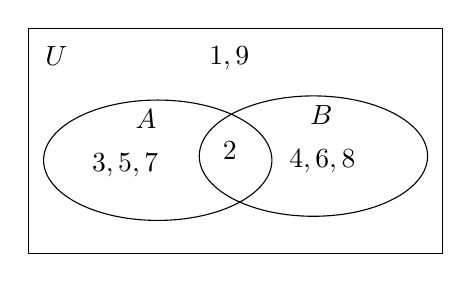
\begin{tikzpicture}[x=0.75pt,y=0.75pt,yscale=-1,xscale=1]
		%uncomment if require: \path (0,300); %set diagram left start at 0, and has height of 300

		%Shape: Rectangle [id:dp7072478037374308] 
		\draw   (247,73) -- (446.4,73) -- (446.4,181.6) -- (247,181.6) -- cycle ;
		%Shape: Ellipse [id:dp7336265334601111] 
		\draw   (254.4,136.6) .. controls (254.4,120.58) and (279.02,107.6) .. (309.4,107.6) .. controls (339.78,107.6) and (364.4,120.58) .. (364.4,136.6) .. controls (364.4,152.62) and (339.78,165.6) .. (309.4,165.6) .. controls (279.02,165.6) and (254.4,152.62) .. (254.4,136.6) -- cycle ;
		%Shape: Ellipse [id:dp8796498546563649] 
		\draw   (329.4,134.6) .. controls (329.4,118.58) and (354.02,105.6) .. (384.4,105.6) .. controls (414.78,105.6) and (439.4,118.58) .. (439.4,134.6) .. controls (439.4,150.62) and (414.78,163.6) .. (384.4,163.6) .. controls (354.02,163.6) and (329.4,150.62) .. (329.4,134.6) -- cycle ;

		% Text Node
		\draw (254,80.4) node [anchor=north west][inner sep=0.75pt]    {$U$};
		% Text Node
		\draw (333,80.4) node [anchor=north west][inner sep=0.75pt]    {$1,9$};
		% Text Node
		\draw (297.5,110.9) node [anchor=north west][inner sep=0.75pt]    {$A$};
		% Text Node
		\draw (381.5,108.9) node [anchor=north west][inner sep=0.75pt]    {$B$};
		% Text Node
		\draw (276.5,132.4) node [anchor=north west][inner sep=0.75pt]    {$3,5,7$};
		% Text Node
		\draw (339.5,126.4) node [anchor=north west][inner sep=0.75pt]    {$2$};
		% Text Node
		\draw (371.5,130.4) node [anchor=north west][inner sep=0.75pt]    {$4,6,8$};


	\end{tikzpicture}
	\caption{}
	\label{fig:Venn}
\end{figure}

\begin{example}
	设 $A 、 B$ 都是不超过 9 的正整数组成的全集 $U$ 的子集, $A \cap B=$ $\{2\},\left(\complement_{U} A\right) \cap\left(\complement_{U} B\right)=\{1,9\},\left(\complement_{U} A\right) \cap B=\{4,6,8\}$, 求 $A \backslash B$.
\end{example}

\begin{analysis}
	直接进行集合间的运算和推理似乎较难入手,但我们可从~\autoref{fig:Venn}中得到解题思路的提示.
\end{analysis}

\begin{solution}
	因为 $\complement_{U}(A \cup B)=\left(\complement_{U} A\right) \cap\left(\complement_{U} B\right)=$ $\{1,9\}$, 所以 $A \cup B=\{2,3,4,5,6,7,8\}$.

	又
	$$
		\begin{aligned}
			A \cap B                              & =\{2\},     \\
			\left(\complement_{U} A\right) \cap B & =\{4,6,8\},
		\end{aligned}
	$$




	所以
	$$
		\begin{aligned}
			B & =U \cap B=\left(A \cup \complement_{U} A\right) \cap B             \\
			  & =(A \cap B) \cup\left(\left(\complement_{U} A\right) \cap B\right) \\
			  & =\{2,4,6,8\} .
		\end{aligned}
	$$

	所以, $A \backslash B=(A \cup B) \backslash B=\{3,5,7\}$.

\end{solution}

\begin{example}
	已知集合 $A=\{(x, y) \mid a x+y=1\}, B=\{(x, y) \mid x+a y=1\}$, $C=\left\{(x, y) \mid x^{2}+y^{2}=1\right\}$. 问:

	(1) 当 $a$ 取何值时, $(A \cup B) \cap C$ 为含有两个元素的集合?

	(2) 当 $a$ 取何值时, $(A \cup B) \cap C$ 为含有三个元素的集合?

\end{example}

\begin{analysis}
	因为 $(A \cup B) \cap C=(A \cap C) \cup(B \cap C)$, 故可从解 $A \cap C$ 及 $B \cap C$ 对应的方程组入手.
\end{analysis}

\begin{solution}
	$(A \cup B) \cap C=(A \cap C) \cup(B \cap C), A \cap C$ 与 $B \cap C$ 分别为方程组

	(i) $\left\{\begin{array}{l}a x+y=1, \\ x^{2}+y^{2}=1,\end{array}\right.$
	\qquad
	(ii) $\left\{\begin{array}{l}x+a y=1, \\ x^{2}+y^{2}=1\end{array}\right.$

	的解集.

	由 (i) 解得 $(x, y)=(0,1),\left(\frac{2 a}{1+a^{2}}, \frac{1-a^{2}}{1+a^{2}}\right)$;

	由 (ii) 解得 $(x, y)=(1,0),\left(\frac{1-a^{2}}{1+a^{2}}, \frac{2 a}{1+a^{2}}\right)$.

	(1) 使 $(A \cup B) \cap C$ 恰有两个元素的情况只有两种可能:

	\ding{172} $\left\{\begin{array}{l}\frac{2 a}{1+a^{2}}=0, \\ \frac{1-a^{2}}{1+a^{2}}=1 ;\end{array}\right.$
	\qquad
	\ding{173} $\left\{\begin{array}{l}\frac{2 a}{1+a^{2}}=1 \\ \frac{1-a^{2}}{1+a^{2}}=0 .\end{array}\right.$\\
	由\ding{172}得 $a=0$; 由\ding{173}得 $a=1$.

	故当 $a=0$ 或 1 时, $(A \cup B) \cap C$ 恰有两个元素.

	(2) 使 $(A \cup B) \cap C$ 恰有三个元素的情况是
	$$
		\frac{2 a}{1+a^{2}}=\frac{1-a^{2}}{1+a^{2}}
	$$

	解得 $a=-1 \pm \sqrt{2}$.

	故当 $a=-1 \pm \sqrt{2}$ 时, $(A \cup B) \cap C$ 恰有三个元素.
\end{solution}

\begin{example}\label{ex:1.2.3}
	设 $n \in \mathbb{N}$, 且 $n \geqslant 15, A 、 B$ 都是 $\{1,2, \cdots, n\}$ 的真子集, $A \cap B=\varnothing$,且 $\{1,2, \cdots, n\}=A \cup B$. 证明: $A$ 或者 $B$ 中必有两个不同数的和为完全平方数.
\end{example}

\begin{proof}
	由题设, $\{1,2, \cdots, n\}$ 的任何元素必属于且只属于它的真子集 $A$ 、 $B$ 之一. 假设结论不真, 则存在如题设的 $\{1,2, \cdots, n\}$ 的真子集 $A 、 B$, 使得无论是 $A$ 还是 $B$ 中的任何两个不同的数的和都不是完全平方数.

	不妨设 $1 \in A$, 则 $3 \notin A$. 否则 $1+3=2^{2}$, 与假设矛盾, 所以 $3 \in B$. 同样, $6 \notin B$, 所以 $6 \in A$. 这时 $10 \notin A$, 即 $10 \in B$. 因 $n \geqslant 15$, 而 15 或者在 $A$ 中, 或者在 $B$ 中,但当 $15 \in A$ 时, 因 $1 \in A, 1+15=4^{2}$, 矛盾; 当 $15 \in B$ 时,因 $10 \in B, 10+15=5^{2}$, 仍然矛盾. 因此假设不真, 即 $A$ 或者 $B$ 中必有两个不同数的和为完全平方数.
\end{proof}

\begin{note}
	由 $A 、 B$ 地位对称, 在上面的解法中我们采用了“不妨设 $1 \in A$ ”这种技巧, 有效简化了解题过程.
\end{note}

~\autoref{ex:1.2.3}实际上给出了一个关于集合的方程组:
$$
	\left\{\begin{array}{l}
		A \cup B=\{1,2, \cdots, n\} \\
		A \cap B=\varnothing
	\end{array}\right.
$$

如果交换 $A 、 B$ 算两组解 (有序解) ,那么这个方程组有多少组有序解呢?

设 $U=\{1,2, \cdots, n\}$, 由 $A \cup B=U, A \cap B=\varnothing$, 知 $A$ 与 $B$ 互补, 对于 $A \subseteq U$, 可取 $B=\complement_{U} A$. 故上述集合方程的有序解的个数为 $2^{n}$.

\begin{example}
	设集合 $S$ 含有 $n$ 个元素, $A_{1}, A_{2}, \cdots, A_{k}$ 是 $S$ 的不同子集, 它们两两的交集非空, 而 $S$ 的其他子集不能与 $A_{1}, A_{2}, \cdots, A_{k}$ 都相交. 求证: $k=2^{n-1}$.
\end{example}

\begin{analysis}
	$S$ 有 $2^{n}$ 个子集, 将两个互为补集的子集作为一组, 则可将 $2^{n}$ 个子集分成 $2^{n-1}$ 个组, 记为 $\left\{A_{i}^{\prime}, B_{i}^{\prime}\right\}, i=1,2, \cdots, 2^{n-1}$, 显然 $A_{i}$ 只能选取每组中的一个子集.
\end{analysis}

\begin{proof}
	设 $a \in S$. 因为 $|S|=n$, 故 $S$ 的子集中含 $a$ 的子集有 $2^{n-1}$ 个. 显然\\
	它们两两的交非空. 所以, $k \geqslant 2^{n-1}$.

	又可将 $S$ 的 $2^{n}$ 个子集分成 $2^{n-1}$ 组, 每组有两个集合, 它们互为补集. 若 $k>2^{n-1}$, 则必有两个集合 $A_{i} 、 A_{j}(i \neq j)$ 来自上述同一组, 但 $A_{i} \cap A_{j}=\varnothing$, 与题意不符. 所以, $k=2^{n-1}$.
\end{proof}

\begin{example}
	已知集合 $A$ 中包含 2016 个点且无四点共线. 证明: 在集合 $A$ 中存在一个至少有 63 个点的子集 $B$, 使得 $B$ 中无三点共线.
\end{example}

\begin{analysis}
	自然,我们应该考虑集合 $A$ 中无三点共线的元素个数最多的子集, 设 $B$ 就是一个这样的子集, 那么集合 $A \backslash B$ 中任何一点都与集合 $B$ 中某两点构成三点共线,即 $A \backslash B$ 中任何一点对应集合 $B$ 中一个与之组成三点共线的二元子集, 且 $A \backslash B$ 中不同点对应 $B$ 中不同二元子集,故 $B$ 中二元子集的数量不少于 $A \backslash B$ 中元素的数量.
\end{analysis}

\begin{proof}
	令 $B \subseteq A$ 且 $B$ 为无三点共线的最大的子集.

	由于 $B$ 为满足条件的最大集合, 于是, 集合 $A \backslash B$ 中任意一点与集合 $B$ 中的某两个点共线.

	又集合 $A$ 中无四点共线,则过集合 $B$ 中的两个点的每条直线最多包含集合 $A \backslash B$ 中的一个点.

	故集合 $A \backslash B$ 中的点的数目不大于集合 $B$ 中的点对的数目.

	记 $|B|=k$, 则集合 $A \backslash B$ 中点的数目为 $2016-k$, 集合 $B$ 中点对的数目为 $\frac{k(k-1)}{2}$. 所以
	$$
		2016-k \leqslant \frac{(k-1) k}{2}
	$$

	解得 $k \geqslant 63$ 或 $k \leqslant-64$ (负值舍去).

	因此,集合 $B$ 中至少有 63 个点.
\end{proof}

\begin{example}
	令 $S=\{1,2, \cdots, 2014\}$. 对于每个非空子集 $T \subseteq S$, 可选择 $T$ 的一个元素作为该集合的代表元. 求将集合 $S$ 的每个非空子集选取一个代表元的不同方式种数, 每种方式须满足对于每个子集 $D \subseteq S$, 若 $D$ 为非空子集 $A$, $B, C \subseteq S$ 的无交并(即子集 $A 、 B 、 C$ 两两不交且并集为 $D$ ), 则集合 $D$ 的代表元至少为 $A 、 B 、 C$ 中的一个代表元.
\end{example}

\begin{solution}
	选取方式有 $108 \times 2014!$ 种.

	用 $r(A)$ 表示集合 $A$ 的代表元, $a_{n}$ 表示当 $S=\{1,2, \cdots, n\}$ 时符合题意的安排方式的种数.

	先计算四元集的情形.

	记 $Y=\left\{y_{1}, y_{2}, y_{3}, y_{4}\right\}$. 则有四种不同方式选出 $r(Y)$, 不妨设 $y_{1}=$ $r(Y)$.

	由 $\left\{y_{1}, y_{2}, y_{3}, y_{4}\right\}=\left\{y_{1}, y_{2}\right\} \cup\left\{y_{3}\right\} \cup\left\{y_{4}\right\}$, 则只能 $r\left(\left\{y_{1}, y_{2}\right\}\right)=$ $y_{1} \cdot$

	类似地, $r\left(\left\{y_{1}, y_{3}\right\}\right)=r\left(\left\{y_{1}, y_{4}\right\}\right)=y_{1}$.

	此时, 只有
	$$
		\begin{aligned}
			 & \left\{y_{1}, y_{2}, y_{3}\right\} 、\left\{y_{1}, y_{2}, y_{4}\right\} 、\left\{y_{1}, y_{3}, y_{4}\right\} 、              \\
			 & \left\{y_{2}, y_{3}, y_{4}\right\} 、\left\{y_{2}, y_{3}\right\} 、\left\{y_{2}, y_{4}\right\} 、\left\{y_{3}, y_{4}\right\}
		\end{aligned}
	$$

	的代表元无法确定, 且可以为集合内的任意一个元素,故有 $3^{4} \times 2^{3}$ 种.

	从而, $a_{4}=4 \times 3^{4} \times 2^{3}=108 \times 4!$.

	对于 $n \geqslant 5$, 只要证明 $a_{n}=n a_{n-1}$.

	记全集 $S$ 的代表元 $r(S)=k$, 则 $k$ 有 $n$ 种选择方式.

	若 $T$ 为含 $k$ 的元素个数至多为 $n-2$ 的子集, 则集合 $S$ 可写成 $T$ 与另两个非空子集的无交并.

	故 $r(T)=k$.

	设 $T$ 为含 $k$ 的 $n-1$ 元子集.

	若 $r(T)=m \neq k$, 则 $T$ 可写成 $\{m, k\}$ 与另两个子集的无交并.

	从而, $r(\{m, k\})=m$, 这与之前的含 $k$ 的元素个数至多是 $n-2$ 的子集的代表元为 $k$ 的结论矛盾.

	故含 $k$ 的所有子集代表元必为 $k$.

	从而, 将 $n$ 降为了 $n-1$ 的情形可得递推式 $a_{n}=n a_{n-1}$.
\end{solution}

\begin{note}
	正确理解集合 $D$ 的代表元的特殊性是解本例的关键. 设 $D=\left\{y_{1}\right.$, $\left.y_{2}, y_{3}, y_{4}\right\}, A=\left\{y_{1}, y_{2}\right\}, B=\left\{y_{3}\right\}, C=\left\{y_{4}\right\}$, 且 $r(A)=y_{1}$, 则 $D$ 的代表元不能为 $y_{2}$; 当然, 若 $r(A)=y_{2}$, 则 $D$ 的代表元不能为 $y_{1}$.
\end{note}

\begin{example}
	有 1987 个集合,每个集合有 45 个元素,任意两个集合的并集有 89 个元素,问此 1987 个集合的并集有多少个元素?
\end{example}

\begin{analysis}
	由每个集合有 45 个元素,且任意两个集合的并集有 89 个元素知,任意两个集合有且只有一个公共元素.
\end{analysis}

\begin{solution}
	显然可以由题设找到这样的 1987 个集合, 它们都含有一个公共元素 $a$, 而且每两个集合不含 $a$ 以外的公共元素.

	下面,我们来排除其他可能性.

	由任意两个集合的并集有 89 个元素可知, 1987 个集合中的任意两个集合有且只有一个公共元素, 则容易证明这 1987 个集合中必有一个集合 $A$ 中的元素 $a$ 出现在 $A$ 以外的 45 个集合中, 设为 $A_{1}, A_{2}, \cdots, A_{45}$, 其余的设为 $A_{46}, A_{47}, \cdots, A_{1986}$.

	设 $B$ 为 $A_{46}, A_{47}, \cdots, A_{1986}$ 中的任一个集合, 且 $a \notin B$, 由题设 $B$ 和 $A$, $A_{1}, A_{2}, \cdots, A_{45}$ 都有一个公共元素, 且此 46 个元素各不相同, 故 $B$ 中有 46 个元素,与题设矛盾. 所以这 1987 个集合中均含有 $a$.

	故所求结果为 $1987 \times 44+1=87429$,即这 1987 个集合的并集有 87429 个元素.
\end{solution}

\begin{note}
	在这里我们先设计一种符合题设的特殊情形, 然后再排除其他可能的情形, 从而达到解题目的. 这是一种“先猜后证”的解题策略.
\end{note}

\begin{example}
	将集合 $M=\{1,2, \cdots, 100\}$ 中任意 67 个数染成红色, 另 33 个数染成蓝色. 若集合 $M$ 存在形如
	$$
		A_{i, k}=\{i, i+1, \cdots, i+3 k-1\}(1 \leqslant k \leqslant 33,1 \leqslant i \leqslant 101-3 k)
	$$

	的子集恰有 $2 k$ 个数被染成红色, 另 $k$ 个数被染成蓝色, 求 $k$ 的最大值.
\end{example}

\begin{solution}
	首先, 若将集合 $M$ 中从 $18 \sim 84$ 这 67 个数染成红色, 其他的数染成蓝色, 则当 $17<k \leqslant 33$ 时, 显然, 不存在满足题设条件的子集 $A_{i, k}$. 故 $k_{\max } \leqslant$ 17.

	下面证明 $: k_{\text {max }}=17$.

	事实上,当 $1 \leqslant i \leqslant 49$ 时,集合
	$$
		A_{i, 17}=\{i, i+1, \cdots, i+50\} \text { 与 } A_{i+1,17}=\{i+1, i+2, \cdots, i+51\}
	$$
	中红色数的个数至多相差 1.

	(i) $i$ 与 $i+51$ 同色.

	则集合 $A_{i, 17} 、 A_{i+1,17}$ 的红色数个数相等;

	(ii) $i$ 为红、 $i+51$ 为蓝.

	则集合 $A_{i, 17}$ 的红色数个数比集合 $A_{i+1,17}$ 的红色数个数多 1 ;

	(iii) $i$ 为蓝、 $i+51$ 为红.

	则集合 $A_{i, 17}$ 的红色数个数比集合 $A_{i+1,17}$ 的红色数个数少 1 .

	考虑下面两个集合
	$$
		\begin{gathered}
			A_{1,17}=\{1,2, \cdots, 51\} \\
			A_{50,17}=\{50,51, \cdots, 100\}
		\end{gathered}
	$$

	若 $A_{1,17} 、 A_{50,17}$ 中至少有一个集合恰好有 34 个数染成红色, 则结论成立.

	设集合 $A_{1,17} 、 A_{50,17}$ 的红色数个数不是 34.\\
	记 $A=A_{1,17} \cap A_{50,17}=\{50,51\}$.

	下面分三种情形讨论.

	(1)当集合 $A$ 中两个数均为红色时,由抽屉原则,知集合
	$$
		A_{1,17} \backslash A=\{1,2, \cdots, 49\} \text { 与 } A_{50,17} \backslash A=\{52,53, \cdots, 100\}
	$$

	中必有一个的红色数个数不少于 33.

	由对称性, 不妨设集合 $A_{1,17} \backslash A$ 中的红色数个数不少于 33 , 则集合 $A_{1,17}$中的红色数个数不少于 35 ,集合 $A_{50,17}$ 中的红色数个数不多于 33.

	由前面证明, 知集合 $A_{1.17}, A_{2,17}, \cdots, A_{50,17}$ 中至少有一个其红色数的个数恰为 33 .

	(2) 当集合 $A$ 中两个数为 1 红 1 蓝时, 则集合 $A_{1,17} \backslash A$ 与 $A_{50,17} \backslash A$ 中红色数的个数一个多于 33 ,一个少于 33 . 同上可证.

	(3) 当集合 $A$ 中两个数都为蓝色时, 则集合 $A_{1,17} \backslash A$ 与 $A_{50,17} \backslash A$ 中红色数的个数一个不少于 35, 一个不多于 33 . 同上可证.

	综上, $k_{\max }=17$.
\end{solution}

\begin{example}
	设 $m, n \in \mathbb{Z}_{+}$, 已知有 $n$ 堆金币,第 $i(1 \leqslant i \leqslant n)$ 堆中含有 $a_{i}\left(a_{i}>\right.$ 0) 枚. 鲍勃和爱丽丝按照如下步骤进行游戏:

		第一步:鲍勃选择集合 $\{1,2, \cdots, m\}$ 的非空子集 $B_{1}, B_{2}, \cdots, B_{n}$;

		第二步:在得知鲍勃第一步选择的集合 $B_{1}, B_{2}, \cdots, B_{n}$ 后, 爱丽丝选择集合 $\{1,2, \cdots, m\}$ 的一个非空子集 $S ;$

		第三步:若 $B_{i} \cap S$ 的元素个数为偶数, 则第 $i$ 堆的金币就归鲍勃所有,否则,归爱丽丝所有.

		证明: 无论鲍勃如何选择集合 $B_{1}, B_{2}, \cdots, B_{n}$, 爱丽丝总能选择一个集合使得她得到的金币总数比鲍勃多.
\end{example}

\begin{proof}
	游戏结束时, 爱丽丝获得的金币数多于鲍勃获得的金币数当且仅当
	$$
		\sum_{i=1}^{n}(-1)^{\left|B_{i} \cap S\right|} a_{i}<0
	$$

	否则,对任意的非空集合 $S$ 有
	$$
		\sum_{i=1}^{n}(-1)^{\left|B_{i} \cap S\right|} a_{i}>0
	$$

	显然, 当 $S=\varnothing$ 时,
	$$
		\sum_{i=1}^{n}(-1)^{\left|B_{i} \cap s\right|} a_{i}=\sum_{i=1}^{n} a_{i}>0
	$$

	故
	\begin{equation}
		\sum_{S \subseteq\{1,2, \cdots, m\}} \sum_{i=1}^{n}(-1)^{\left|B_{i} \cap s\right|} a_{i}>0
		\label{eq:鲍勃和爱丽丝}
	\end{equation}

	当 $B$ 是 $\{1,2, \cdots, m\}$ 的非空子集时, 考虑 $\sum_{S \subseteq\{1,2, \cdots, m\}}(-1)^{|B \cap S|}$.记 $S=C \cup D$, 其中, $C=S \backslash B, D=S \cap B, C \cap D=\varnothing$. 则
	$$
		\begin{aligned}
			  & \sum_{S \subseteq\{1,2, \ldots, m\}}(-1)^{|B \cap S|}                                 \\
			= & \sum_{C \subseteq\{1,2, \ldots, m \nmid B} \sum_{D \subseteq B}(-1)^{|B \cap(C U D)|} \\
			= & \sum_{C \subseteq\{1,2, \cdots, m \backslash B} \sum_{D \subseteq B}(-1)^{|D|} .
		\end{aligned}
	$$

	因为 $|B|>0$, 所以,
	$$
		\sum_{D \subseteq B}(-1)^{|D|}=\sum_{r=0}^{|B|}(-1)^{r} \mathrm{C}_{|B|}^{r}=0
	$$

	则对每个非空子集 $B \subseteq\{1,2, \cdots, m\}$ 有
	$$
		\sum_{S \subseteq\{1,2, \ldots, m\}}(-1)^{|B \cap S|}=0
	$$

	故
	$$
		\sum_{S \subseteq\{1,2, \ldots, m\}} \sum_{i=1}^{n}(-1)^{\left|B_{i} \cap S\right|} a_{i}=\sum_{i=1}^{n}\left[a_{i} \sum_{S \subseteq\{1,2, \ldots, m\}}(-1)^{\left|B_{i} \cap S\right|}\right]=0
	$$

	与~\autoref{eq:鲍勃和爱丽丝}矛盾.
\end{proof}

\begin{example}
	设 $A$ 是集合 $S=\{1,2, \cdots, 1000000\}$ 的一个恰有 101 个元素的子集. 证明: 在 $S$ 中存在数 $t_{1}, t_{2}, \cdots, t_{100}$, 使得集合
	$$
		A_{j}=\left\{x+t_{j} \mid x \in A\right\}, j=1,2, \cdots, 100
	$$
	中,每两个的交集为空集.
\end{example}
\begin{analysis}
	先弄清楚在什么情况下 $A_{i} \cap A_{j} \neq \varnothing$. 设 $a \in A_{i} \cap A_{j}$, 则 $a=x+$ $t_{i}=y+t_{j}, x, y \in A$. 于是 $t_{i}-t_{j}=y-x$. 这说明选取 $t_{1}, t_{2}, \cdots, t_{100}$ 时, 只要保证其中任意两个之差不等于 $A$ 中任二元素之差即可.
\end{analysis}

\begin{proof}
	考虑集合 $D=\{x-y \mid x, y \in A\}$, 则
	$$
		|D| \leqslant 101 \times 100+1=10101
	$$

	若 $A_{i} \cap A_{j} \neq \varnothing$, 设 $a \in A_{i} \cap A_{i}$, 则 $a=x+t_{i}, a=y+t_{j}$, 其中 $x, y \in$ $A$,则 $t_{i}-t_{j}=y-x \in D$.

	若 $t_{i}-t_{j} \in D$, 即存在 $x, y \in A$, 使得 $t_{i}-t_{j}=y-x$, 从而 $x+t_{i}=y+t_{j}$,即 $A_{i} \cap A_{j} \neq \varnothing$.

	所以, $A_{i} \cap A_{j} \neq \varnothing$ 的充要条件是 $t_{i}-t_{j} \in D$. 于是, 我们只需在集 $S$ 中取出 100 个元素, 使得其中任意两个的差都不属于 $D$.

	下面用递推方法来取出这 100 个元素.

	先在 $S$ 中任取一个元素 $t_{1}$, 再从 $S$ 中取一个 $t_{2}$, 使得 $t_{1} \notin t_{2}+D=\left\{t_{2}+\right.$ $x \mid x \in D\}$, 这是因为取定 $t_{1}$ 后, 至多有 10101 个 $S$ 中的元素不能作为 $t_{2}$, 从而在 $S$ 中存在这样的 $t_{2}$, 若已有 $k(\leqslant 99)$ 个 $S$ 中的元素 $t_{1}, t_{2}, \cdots, t_{k}$ 满足要求, 再取 $t_{k+1}$, 使得 $t_{1}, t_{2}, \cdots, t_{k}$ 都不属于 $t_{k+1}+D=\left\{t_{k+1}+x \mid x \in D\right\}$. 这是因为 $t_{1}, t_{2}, \cdots, t_{k}$ 取定后, 至多有 $10101 k \leqslant 999999$ 个 $S$ 中的数不能作为 $t_{k+1}$,故在 $S$ 中存在满足条件的 $t_{k+1}$. 所以, 在 $S$ 中存在 $t_{1}, t_{2}, \cdots, t_{100}$, 其中任意两个的差都不属于 $D$.

	综上所述, 命题得证.
\end{proof}

\begin{note}
	条件 $|S|=10^{6}$ 可以改小一些. 一般地, 我们有如下更强的结论:

	若 $A$ 是 $S=\{1,2, \cdots, n\}$ 的一个 $k$ 元子集, $m$ 为正整数,且 $m$ 满足条件 $n>(m-1)\left(\mathrm{C}_{k}^{2}+1\right)$, 则存在 $S$ 中的元素 $t_{1}, t_{2}, \cdots, t_{m}$, 使得 $A_{j}=\left\{x+t_{j} \mid\right.$ $x \in A\}, j=1,2, \cdots, m$ 中任意两个的交集为空集.

	有兴趣者可自己证明.
\end{note}

\section{有限集的阶}
我们知道集合可以分为有限集和无限集两类. 研究无限集元素的“数目”是一个困难而有趣的问题, 最出名的就是所谓“连续统假设”, 但它不是我们的话题. 我们要讨论的问题仅与有限集有关.
\subsection{有限集的阶}
有限集 $A$ 的元素的数目叫做这个集合的阶, 记作 $|A|$ (或 $n(A))$.
\begin{example}
	设集合 $A=\{a \mid 1 \leqslant a \leqslant 2000, a=4 k+1, k \in \mathbb{Z}\}$, 集合 $B=$ $\{b \mid 1 \leqslant b \leqslant 3000, b=3 k-1, k \in \mathbb{Z}\}$. 求 $|A \cap B|$.
\end{example}

\begin{analysis}
	令 $4 k+1=3 m-1$, 得 $m=\frac{4 k+2}{3}=k+1+\frac{k-1}{3}$. 因 $m \in \mathbb{Z}$, 所以 $3 \mid k-1$. 令 $k-1=3 r, r \in \mathbb{Z}$, 得 $m=4 r+2$. 这时 $b=12 r+5$, 故 $A \cap B$的元素是形如 $12 r+5$ 的整数.
\end{analysis}

\begin{solution}
	形如 $4 k+1$ 的数可分为 3 类:
	$$
		12 l+1,12 l+5,12 l+9(l \in \mathbb{Z})
	$$

	其中只有形如 $12 l+5$ 的数是形如 $3 k-1$ 的数. 令
	$$
		1 \leqslant 12 l+5 \leqslant 2000(l \in \mathbb{Z})
	$$

	得 $0 \leqslant l \leqslant 166$. 所以, $A \cap B=\{5,17, \cdots, 1997\}$.

	所以, $|A \cap B|=167$.
\end{solution}

\begin{note}
	上例, 我们是采用列举出集合的全部元素的办法来求其元素的数目. 对于一些较为复杂的集合, 这种方法是很难奏效的, 这时必须另辟蹊径.
\end{note}

\begin{example}
	给定正整数 $n(n \geqslant 2)$. 称集合 $S(|S|=n)$ 的三个互不相同的子集 $S_{i} 、 S_{j} 、 S_{k}$ 为一个“三角形”. 定义
	$$
		\left|\left(S_{i} \cap S_{j}\right) \cup\left(S_{j} \cap S_{k}\right) \cup\left(S_{k} \cap S_{i}\right)\right|
	$$
	为这个三角形的“周长”. 试求周长为 $n$ 的三角形的个数.
\end{example}

\begin{analysis}
	命题等价于集合 $S$ 有多少组三个互不相同的子集 $S_{i} 、 S_{i} 、 S_{k}$, 使
	$$
		\left(S_{i} \cap S_{j}\right) \cup\left(S_{j} \cap S_{k}\right) \cup\left(S_{k} \cap S_{i}\right)=S
	$$
\end{analysis}

\begin{solution}
	令 $T_{1}=\left(S_{i} \cap S_{j}\right) \backslash S_{k}, T_{2}=\left(S_{i} \cap S_{j}\right) \backslash S_{i}, T_{3}=\left(S_{k} \cap S_{i}\right) \backslash S_{j}$, $T_{4}=S_{i} \cap S_{j} \cap S_{k}$.

	本题等价于求有多少种方式将数 $1,2, \cdots, n$ 放入集合 $T_{1} 、 T_{2} 、 T_{3} 、 T_{4}$中,使得 $S_{i} 、 S_{i} 、 S_{k}$ 互不相同.

	首先, 将 $1,2, \cdots, n$ 放入集合 $T_{1} 、 T_{2} 、 T_{3} 、 T_{4}$ 中,共有 $4^{n}$ 种方法.

	其次, 若 $S_{i}=S_{j}$, 则 $S_{i}=S_{i} \cap S_{j}=S_{j}$. 从而, 将 1, $2, \cdots, n$ 放入集合 $T_{1} 、 T_{4}$ 中, 共有 $2^{\prime \prime}$ 种方法, 这不满足条件.

	类似地, $S_{j}=S_{k}, S_{k}=S_{i}$ 都有 $2^{\prime \prime}$ 种方式不满足条件.

	但是 $S_{i}=S_{j}=S_{k}$ 被多减了两次.

	最后, 再考虑 $S_{i} 、 S_{j} 、 S_{k}$ 的次序.

	故所求的周长为 $n$ 的三角形的个数为 $\frac{1}{6}\left(4^{n}-3 \times 2^{n}+2\right)$.
\end{solution}

\begin{example}
	设 $a_{1}, a_{2}, \cdots, a_{n}$ 为 $1,2, \cdots, n$ 的一个排列, $f_{k}=\mid\left\{a_{i} \mid a_{i}<a_{k}\right.$, $i>k\}\left|, g_{k}=\right|\left\{a_{i} \mid a_{i}>a_{k}, i<k\right\} \mid$, 其中 $k=1,2, \cdots, n$. 证明:
	$$
		\sum_{k=1}^{n} g_{k}=\sum_{k=1}^{n} f_{k}
	$$
\end{example}

\begin{analysis}
	一般来说 $f_{k} \neq g_{k}$, 且分别计算 $f_{k} 、 g_{k}$ 是困难的. 令 $A_{k}=$ $\left\{a_{i} \mid a_{i}<a_{k}, i>k\right\}$, 对 $A_{k}$ 换一种写法: $A_{k}=\left\{\left(a_{i}, a_{k}\right) \mid a_{i}<a_{k}, i>k\right\}$, 显然是合理的. 易知 $k \neq k^{\prime}$ 时, $A_{k} \cap A_{k}{ }^{\prime}=\varnothing$. 所以,
	$$
		\begin{aligned}
			\sum_{k=1}^{n} f_{k} & =\left|A_{1}\right|+\left|A_{2}\right|+\cdots+\left|A_{n}\right|=\left|A_{1} \cup A_{2} \cup \cdots \cup A_{n}\right| \\
			                     & =\left|\left\{\left(a_{i}, a_{j}\right) \mid a_{i}<a_{j}, i>j\right\}\right|
		\end{aligned}
	$$
\end{analysis}

\begin{proof}
	考虑集合 $A=\left\{\left(a_{i}, a_{j}\right) \mid a_{i}<a_{j}, i>j\right\}$ 的元素的数目 $|A|$.

	一方面, 固定 $a_{j}$ 时, $a_{i}$ 的个数为 $f_{j}$. 所以 $|A|=\sum_{j=1}^{n} f_{j}$.

	另一方面, 固定 $a_{i}$ 时, $a_{j}$ 的个数为 $g_{i}$, 所以 $|A|=\sum_{i=1}^{n} g_{i}$.

	所以, $\sum_{k=1}^{n} g_{k}=\sum_{k=1}^{n} f_{k}$.
\end{proof}

\begin{note}
	在这里, 我们没有直接证明 $\sum_{k=1}^{n} g_{k}=\sum_{k=1}^{n} f_{k}$, 而是引入一个中间量 $|A|=\left|\left\{\left(a_{i}, a_{j}\right) \mid a_{i}<a_{j}, i>j\right\}\right|$ 来过渡.
\end{note}

\begin{example}
	在集合 $\{1,2, \cdots, 2 n\}$ 中选取其中 $n$ 个数, 记为 $a_{1}, a_{2}, \cdots, a_{n}\left(a_{1}\right.$ $\left.<a_{2}<\cdots<a_{n}\right)$, 剩下 $n$ 个数记为 $b_{1}, b_{2}, \cdots, b_{n}\left(b_{1}>b_{2}>\cdots>b_{n}\right)$. 证明:
	$$
		\left|a_{1}-b_{1}\right|+\left|a_{2}-b_{2}\right|+\cdots+\left|a_{n}-b_{n}\right|=n^{2}
	$$
\end{example}

\begin{analysis}
	观察如下刻意排序的两组数:
	$$
		\begin{aligned}
			 & a_{1}<a_{2}<\cdots<a_{j}<\cdots<a_{n} \\
			 & b_{1}>b_{2}>\cdots>b_{j}>\cdots>b_{n}
		\end{aligned}
	$$

	不难发现 $a_{j} 、 b_{j}$ 不能同时属于或不属于集合 $\{1,2, \cdots, n\}$. 否则, 不妨设 $a_{j}$, $b_{j} \in\{1,2, \cdots, n\}$, 这时便有 $n+1$ 个不同的数属于集合 $\{1,2, \cdots, n\}$, 这是不可能的.
\end{analysis}

\begin{proof}
	记 $L=\{1,2, \cdots, n\}, H=\{n+1, n+2, \cdots, 2 n\}$. 则 $a_{i} 、 b_{i}(i=$ $1,2, \cdots, n)$ 不能同在集合 $L$ 中, 也不能同在集合 $H$ 中.

	否则, 设 $j \in\{1,2, \cdots, n\}, a_{j} \in L, b_{j} \in L$. 因为 $a_{i}$ 是按照从小到大的顺序排列, $b_{i}$ 是按照从大到小的顺序排列, 所以, 当 $i \leqslant j$ 时, $a_{i} \in L$; 当 $i \geqslant j$时, $b_{i} \in L$. 又所有的数均不相同, 则集合 $L$ 包含 $j$ 个 $a_{i}$ 和 $n-j+1$ 个 $b_{i}$. 于是, 集合 $L$ 中的总元素有 $j+(n-j+1)=n+1$ (个). 矛盾.

	同理,假设 $a_{i} 、 b_{i}$ 同在集合 $H$ 中时,也导出矛盾.

	因此, 对于每一个 $i(i=1,2, \cdots, n)$ 均有
	$$
		\left|a_{i}-b_{i}\right|=\left(h_{i}-l_{i}\right)\left(h_{i} \in H, l_{i} \in L\right) \text {. }
	$$

	故
	$$
		\begin{aligned}
			  & \left|a_{1}-b_{1}\right|+\left|a_{2}-b_{2}\right|+\cdots+\left|a_{n}-b_{n}\right| \\
			= & \left(h_{1}-l_{1}\right)+\left(h_{2}-l_{2}\right)+\cdots+\left(h_{n}-l_{n}\right) \\
			= & \left(h_{1}+h_{2}+\cdots+h_{n}\right)-\left(l_{1}+l_{2}+\cdots+l_{n}\right)       \\
			= & (n+1+n+2+\cdots+2 n)-(1+2+\cdots+n)                                               \\
			= & n^{2} .
		\end{aligned}
	$$
\end{proof}

\begin{note}
	上例看似与集合没有太多联系, 但蕴涵在题设条件中的关键事实: $a_{j} 、 b_{j}$ 不能同时属于或不属于集合 $\{1,2, \cdots, n\}$, 它是由集合 $\{1,2, \cdots$, $n\}$ 的阶决定的.
\end{note}

\begin{example}
	某国家有 $N$ 座城市, 它们中的某些城市有双向的航班连接. 每个航班恰连接两座城市, 没有城市直接连接每个其他城市, 且对于任意两座城市 $A 、 B$, 恰有一种至多存在两个航班从城市 $A$ 到城市 $B$ 的方式飞行. 证明: $N-$ 1 为完全平方数.
\end{example}

\begin{proof}
	设 $a$ 为任意一座城市, 与它连接的城市为 $x_{1}, x_{2}, \cdots, x_{k}$.

	令 $B_{i}(i=1,2, \cdots, k)$ 为异于城市 $a$ 且连接 $x_{i}$ 的所有城市的集合.

	因为从城市 $x_{i}$ 至城市 $x_{j}$ 恰有一种方式飞行至多存在两个航班, 所以, 集合 $B_{1}, B_{2}, \cdots, B_{k}$ 两两无交集.

	考虑两个角标 $i 、 j$ 和任意的城市 $y \in B_{i}$, 由于从城市 $y$ 至 $x_{j}$ 只有一种飞行方式至多存在两个航班且无直飞航班, 则存在唯一的城市 $z \in B_{j}$, 使得城市 $y$ 与 $z$ 有航班连接.

	故每个集合 $B_{i}$ 中的每个元素恰有 $k$ 种上述连接方式, 且所有集合 $B_{i}$ 的元素的个数相同.

	令 $m$ 为集合 $B_{i}$ 中元素的个数, 则 $N=1+k+k m$.

	此外, 考虑某座城市 $b \in B_{1}$, 它与 $x_{1}$ 相连, 恰有一座城市 $c_{i} \in B_{i}(i=2$, $3, \cdots, k)$ 与之相连.

	注意到, 对于 $i=2,3, \cdots, k$, 城市 $x_{i}$ 与城市 $c_{i}$ 相连.

	用同样的方法 (用 $a$ 替换 $b$ ), 知城市 $x_{i}(i=2,3, \cdots, k)$ 有 $k$ 种连接方式,但已知城市 $x_{i}$ 有 $m+1$ 种连接方式, 因此,
	$$
		k=m+1, N-1=k+k m=k^{2} \text {. }
	$$
\end{proof}

\begin{note}
	本例我们是通过引入集合语言,讨论有限集的阶来达到证明的目的的.
\end{note}

\subsection{有关集合阶的不等式}
有些集合虽然不能准确求出其元素的数目,但是我们可以利用不等式来估计其阶的范围.
\begin{example}
	设 $p \geqslant 5$ 是一个素数, $S=\{1,2, \cdots, p-1\}, A=\{a \mid a \in S$, $\left.a^{p-1} \not \equiv 1\left(\bmod p^{2}\right)\right\}$. 证明: $|A| \geqslant \frac{p-1}{2}$.
\end{example}

\begin{analysis}
	如果 $1 \leqslant a \leqslant p-1$, 显然 $1 \leqslant p-a \leqslant p-1$. 将 $a$ 与 $p-a$ 配对,如果 $a^{p-1}$ 与 $(p-a)^{p^{-1}}$ 模 $p^{2}$ 不同余, 则结论成立.
\end{analysis}

\begin{proof}
	设 $a \in S$, 则 $p-a \in S$. 由二项式定理, 有
	$$
		(p-a)^{p-1}-a^{p-1} \equiv-(p-1) a^{p-2} \cdot p \not \equiv 0\left(\bmod p^{2}\right)
	$$

	于是, $a$ 和 $p-a$ 中至少有一个在 $A$ 中, 从而有
	$$
		|A| \geqslant \frac{p-1}{2}
	$$
\end{proof}

\begin{example}
	设 $A_{1}, A_{2}, \cdots, A_{30}$ 是集合 $\{1,2, \cdots, 2003\}$ 的子集,且 $\left|A_{i}\right| \geqslant$ $660, i=1,2, \cdots, 30$. 证明: 存在 $i \neq j, i, j \in\{1,2, \cdots, 30\}$, 使得 $\mid A_{i} \cap$ $A_{j} \mid \geqslant 203$.
\end{example}

\begin{proof}
	不妨设每一个 $A_{i}$ 的元素都为 660 个 (否则去掉一些元素).作一个集合、元素的关系表:表中每一行(除最上面的一行外)分别表示 30 个集合 $A_{1}, A_{2}, \cdots, A_{30}$, 表的 $n$ 列 (最左面一列除外) 分别表示 2003 个元素 1 , $2, \cdots, 2003$. 若 $i \in A_{j}(i=1,2, \cdots, 2003,1 \leqslant j \leqslant 30)$, 则在 $i$ 所在的列与 $A_{j}$ 所在行的交叉处写上 1 , 若 $i \notin A_{j}$, 则写上 0 .

	\begin{center}
		\begin{tabular}{c|ccccc}
			         & 1        & 2        & 3        & $\cdots$ & 2003     \\
			\hline
			$A_{1}$  & $\times$ & $\times$ & $\times$ & $\cdots$ & $\times$ \\
			$A_{2}$  & $\times$ & $\times$ & $\times$ & $\cdots$ & $\times$ \\
			$\cdots$ & $\times$ & $\times$ & $\times$ & $\cdots$ & $\times$ \\
			$A_{30}$ & $\times$ & $\times$ & $\times$ & $\cdots$ & $\times$ \\
		\end{tabular}
	\end{center}

	表中每一行有 660 个 1 ,因此共有 $30 \times 660$ 个 1 . 设第 $j$ 列有 $m_{j}$ 个 1 $(j=1,2, \cdots, 2003)$, 则
	$$
		\sum_{j=1}^{2003} m_{j}=30 \times 660
	$$

	由于每个元素 $j$ 属于 $\mathrm{C}_{m_{j}}^{2}$ 个交集 $A_{s} \cap A_{t}$, 因此
	$$
		\sum_{j=1}^{2003} \mathrm{C}_{m_{j}}^{2}=\sum_{1 \leqslant s<t \leqslant 30}\left|A_{s} \cap A_{t}\right|
	$$

	由柯西不等式, 得
	$$
		\sum_{j=1}^{2003} \mathrm{C}_{m_{j}}^{2}=\frac{1}{2}\left(\sum_{j=1}^{2003} m_{j}^{2}-\sum_{j=1}^{2003} m_{j}\right) \geqslant \frac{1}{2}\left(\frac{1}{2003}\left(\sum_{j=1}^{2003} m_{j}\right)^{2}-\sum_{j=1}^{2003} m_{j}\right)
	$$

	所以,必有 $i \neq j$, 满足
	$$
		\begin{aligned}
			\left|A_{i} \cap A_{j}\right| & \geqslant \frac{1}{\mathrm{C}_{30}^{2}} \times \frac{1}{2}\left(\frac{1}{2003}\left(\sum_{j=1}^{2003} m_{j}\right)^{2}-\sum_{j=1}^{2003} m_{j}\right) \\
			                              & =\frac{660(30 \times 660-2003)}{29 \times 2003}>202
		\end{aligned}
	$$

	从而
	$$
		\left|A_{i} \cap A_{j}\right| \geqslant 203
	$$
\end{proof}

\begin{note}
	本题中所作的表,称为元素、集合从属关系表. 它在讨论涉及多个集合的问题时非常有用.
\end{note}

\begin{example}
	设 $n, k \in \mathbb{N}^{*}$, 且 $k \leqslant n$. 并设 $S$ 是含有 $n$ 个互异实数的集合, $T=\left\{a \mid a=x_{1}+x_{2}+\cdots+x_{k}, x_{i} \in S, x_{i} \neq x_{j}(i \neq j), 1 \leqslant i, j \leqslant k\right\}$. 求证: $|T| \geqslant k(n-k)+1$.
\end{example}

\begin{analysis}
	设 $S_{n}=\left\{s_{1}, s_{2}, \cdots, s_{n-1}, s_{n}\right\}$, 且 $s_{1}<s_{2}<\cdots<s_{n-1}<s_{n}$. 作 $S_{n}$的子集 $S_{n-1}=\left\{s_{1}, s_{2}, \cdots, s_{n-1}\right\}$, 设 $S_{n-1} 、 S_{n}$ 分别对应 $T_{n-1} 、 T_{n}$. 对固定的 $k$ $(k \leqslant n-1)$, 由 $s_{n-1}+s_{n-2}+\cdots+s_{n-k}<s_{n}+s_{n-2}+\cdots+s_{n-k}<s_{n}+s_{n-1}+s_{n-3}$ $+\cdots+s_{n-k}<\cdots<s_{n}+s_{n-1}+\cdots+s_{n-k+1}$, 知 $\left|T_{n}\right| \geqslant\left|T_{n-1}\right|+k$. 而 $k(n-k)+$ $1=k(n-1-k)+k+1$, 这提示我们对 $n$ 进行归纳证明.
\end{analysis}

\begin{proof}
	设 $s_{1}<s_{2}<\cdots<s_{n}$ 是 $S$ 的 $n$ 个元素. 对元素数目 $n$ 使用数学归纳法.

	首先, 当 $k=1$ 和 $k=n$ 时, 结论显然成立. 设 $k \leqslant n-1$, 且结论对 $S_{0}=\left\{s_{1}, s_{2}, \cdots, s_{n-1}\right\}$ 成立, 并设 $T_{0}$ 是当把 $S$ 换成 $S_{0}$ 时与 $T$ 相应的集合. 于是有
	$$
		\begin{gathered}
			\left|T_{0}\right| \geqslant k(n-k-1)+1 . \\
			\text { 令 } x=s_{n}+s_{n-1}+\cdots+s_{n-k} \text {, 并令 } y_{i}=x-s_{n-i}, i=0,1, \cdots, k .
		\end{gathered}
	$$

	显然 $y_{i} \in T$, 且有 $y_{0}<y_{1}<y_{2}<\cdots<y_{k}$. 因为 $y_{0}$ 是 $T_{0}$ 中的最大元素,所以
	$$
		y_{i} \in T, y_{i} \notin T_{0}, i=1,2, \cdots, k
	$$

	故有
	$$
		|T| \geqslant\left|T_{0}\right|+k \geqslant k(n-k-1)+1+k=k(n-k)+1
	$$

	这就完成了归纳证明.
\end{proof}

\begin{example}
	设集合 $F$ 是一个非空有限的整数集, $n$ 为正整数, 满足

	(1) 对任意的 $x \in F$, 均有
	$$
		x=y+z(y, z \in F) \text {; }
	$$

	(2) 若 $1 \leqslant k \leqslant n, x_{1}, x_{2}, \cdots, x_{k} \in F$, 则 $x_{1}+x_{2}+\cdots+x_{k} \neq 0$.证明:集合 $F$ 中至少含有 $2 n+2$ 个互异的元素.
\end{example}

\begin{proof}
	由已知条件 (2)得 $0 \notin F$.

	假设集合 $F$ 只包含正整数. 设 $x$ 是集合 $F$ 中最小的元素. 则由 $x=y+$ $z(y, z>0)$, 知 $y<x, z<x$, 矛盾. 因此, 集合 $F$ 包含负整数. 同理, 集合 $F$也不能只包含负整数.

	假设已经从集合 $F$ 中选出 $k$ 个正整数, 记为 $x_{1}, x_{2}, \cdots, x_{k}$. 所以, $0<x_{k}=y+z(y, z \in F)$.

	不妨设 $y>0$, 则记为 $y$ 为 $x_{k+1}$.

	继续以这样的方式选出集合 $F$ 中的正元素 $x_{1}, x_{2}, \cdots$ (允许相同).

	由 $F$ 是有限集,知存在正整数 $i<j$,使得 $x_{i}, x_{i+1}, \cdots, x_{j-1}$ 互不相同, 且 $x_{j}=x_{i}$.

	于是, 存在 $z_{i}, z_{i+1}, \cdots, z_{j-1} \in F$, 使得
	$$
		\begin{aligned}
			 & x_{i}=x_{i+1}+z_{i},     \\
			 & x_{i+1}=x_{i+2}+z_{i+1}, \\
			 & \cdots                   \\
			 & x_{j-1}=x_{j}+z_{j-1} .
		\end{aligned}
	$$

	因为 $x_{i}=x_{j}$, 所以, $z_{i}+z_{i+1}+\cdots+z_{j-1}=0$.

	由题设得 $j-i>n$.

	又因为 $x_{i}, x_{i+1}, \cdots, x_{j-1}$ 互不相同, 所以, 集合 $F$ 中包含至少 $j-i \geqslant n+$ 1 个正整数.

	同理,集合 $F$ 中包含至少 $n+1$ 个负整数.

	从而, 集合 $F$ 中至少含有 $2 n+2$ 个互异的元素.
\end{proof}

\begin{example}
	设 $A$ 是一个有限实数集, $A_{1}, A_{2}, \cdots, A_{n}$ 是 $A$ 的非空子集, 满足下列条件:

	(1) $A$ 中所有元素之和为 0 ;

	(2) 对任意 $x_{i} \in A_{i}(i=1,2, \cdots, n)$, 都有 $x_{1}+x_{2}+\cdots+x_{n}>0$.

	证明: 存在 $1 \leqslant i_{1}<i_{2}<\cdots<i_{k} \leqslant n$, 使得
	$$
		\left|A_{i_{1}} \cup A_{i_{2}} \cup \cdots \cup A_{i_{k}}\right|<\frac{k}{n}|A|
	$$

	这里 $|X|$ 表示有限集合 $X$ 的元素个数.
\end{example}

\begin{proof}
	设 $A=\left\{a_{1}, a_{2}, \cdots, a_{m}\right\}, a_{1}>a_{2}>\cdots>a_{m}$. 则由条件 (1) 知 $a_{1}+a_{2}+\cdots+a_{m}=0$. 考虑每个 $A_{i}$ 中的最小数, 并设 $A_{1}, A_{2}, \cdots, A_{n}$ 中恰有 $k_{i}$ 个集合的最小数为 $a_{i}, i=1,2, \cdots, m$. 则有
	$$
		k_{1}+k_{2}+\cdots+k_{m}=n
	$$

	且由条件 (2) 知
	$$
		k_{1} a_{1}+k_{2} a_{2}+\cdots+k_{m} a_{m}>0
	$$

	对 $s=1,2, \cdots, m-1$, 共有 $k_{1}+k_{2}+\cdots+k_{s}$ 个集合, 其最小数 $\geqslant a_{s}$. 故这些集合的并集包含在 $\left\{a_{1}, a_{2}, \cdots, a_{s}\right\}$ 中, 元素个数不超过 $s$.

	下证存在 $s \in\{1,2, \cdots, m-1\}$, 使得 $k=k_{1}+k_{2}+\cdots+k_{s}>\frac{s n}{m}$.\\
	用反证法, 设对于 $s=1,2, \cdots, m-1$, 都有
	$$
		k_{1}+k_{2}+\cdots+k_{s} \leqslant \frac{s n}{m}
	$$

	由阿贝尔 (Abel)变换可知 (注意 $a_{s}-a_{s+1}>0,1 \leqslant s \leqslant m-1$)
	$$
		\begin{aligned}
			0<\sum_{j=1}^{m} k_{j} a_{j} & =\sum_{s=1}^{m-1}\left(a_{s}-a_{s+1}\right)\left(k_{1}+k_{2}+\cdots+k_{s}\right)+a_{m}\left(k_{1}+k_{2}+\cdots+k_{m}\right) \\
			                             & \leqslant \sum_{s=1}^{m-1}\left(a_{s}-a_{s+1}\right) \frac{s n}{m}+a_{m} n=\frac{n}{m} \sum_{j=1}^{m} a_{j}=0,
		\end{aligned}
	$$

	矛盾. 对于这一 $s$, 取 $A_{1}, A_{2}, \cdots, A_{n}$ 中最小数 $\geqslant a_{s}$ 的那些集合, 记为 $A_{i_{1}}$, $A_{i_{2}}, \cdots, A_{i_{k}}$. 则由上述的结果可知, 这些子集共有 $k=k_{1}+k_{2}+\cdots+k_{s}>\frac{s n}{m}$个,且它们的并集的元素个数不超过 $s$, 即
	$$
		\left|A_{i_{1}} \cup A_{i_{2}} \cup \cdots \cup A_{i_{k}}\right| \leqslant s<\frac{k m}{n}=\frac{k}{n}|A|
	$$
\end{proof}

\section{子集族}
我们可以将某些集合取来作为元素构成一个新的集合, 如 $A^{*}=\{\{1\}$, $\{0,1\},\{0\}, \varnothing\}$ 就是一个含有 4 个元素 $\{1\}, \{0,1\}, \{0\}, \varnothing$ 的集合. 一般地, 将集合 $M$ 的若干子集作为元素构成的集合 $M^{*}$ 叫做原集合的一个子集族. 例如前面的 $A^{*}$ 就是二元集 $A=\{0,1\}$ 的全部子集所构成的子集族. 子集族 $M^{*}$ 中所含原来集合的子集的数目叫做该子集族的阶, 记作 $\left|M^{*}\right|$. 例如子集族 $A^{*}$ 的阶为 4 , 即 $\left|A^{*}\right|=4$.

根据已知条件求子集族的阶或包含子集族中所有子集的集合的阶, 是较常见的一类集合问题.

\begin{example}
	已知集合 $A=\{1,2, \cdots, 10\}$. 求集合 $A$ 的具有下列性质的子集个数: 每个子集至少含有 2 个元素, 且每个子集中任何两个元素的差的绝对值大于 1 .
\end{example}

\begin{analysis}
	集合 $A$ 有 $2^{10}-1$ 个非空子集, 逐一考察的工作只有交给计算机.我们先来看看比 $A$ 的元素少一些的集合的情形. 记集合 $A_{i}$ 符合条件的子集族为 $A_{i}^{*}, \left|A_{i}^{*}\right|=a_{i}$.
	$$
		\begin{aligned}
			 & A_{1}=\{1\}, A_{1}^{*}=\varnothing, a_{1}=0                         \\
			 & A_{2}=\{1,2\}, A_{2}^{*}=\varnothing, a_{2}=0 ;                     \\
			 & A_{3}=\{1,2,3\}, A_{3}^{*}=\{\{1,3\}\}, a_{3}=1                     \\
			 & A_{4}=\{1,2,3,4\}, A_{4}^{*}=\{\{1,3\},\{1,4\},\{2,4\}\}, a_{4}=3 ; \\
			 & A_{5}=\{1,2,3,4,5\}, A_{5}^{*}=\{\{1,3\},\{1,4\},\{2,4\},\{1,3,5\}  \\
			 & \{1,5\},\{2,5\},\{3,5\}\}, a_{5}=7 .
		\end{aligned}
	$$

	我们来考察写出 $A_{5}^{*}$ 的过程, 这可以分作两步: 第一步写出 $A_{4}^{*}$ 的全部元素, 它们都不含元素 5 ;第二步写出含 5 的子集, 它们是在 $A_{3}^{*}$ 的元素中添 5 所成,或者是含 5 的二元子集, 即 $a_{5}=a_{4}+a_{3}+3$. 其实对 $A_{4}^{*} 、 A_{3}^{*}$ 有类似的\\
	结论: $a_{4}=a_{3}+a_{2}+2, a_{3}=a_{2}+a_{1}+1$. 我们可以将这个作法推广到一般.
\end{analysis}

\begin{solution}
	设 $a_{n}$ 是集合 $\{1,2, \cdots, n\}$ 的具有题设性质的子集个数.

	对于集合 $\{1,2, \cdots, n, n+1, n+2\}$, 具有题设性质的子集可分为两类:第一类子集不包含 $n+2$, 它们是集合 $\{1,2, \cdots, n, n+1\}$ 的全部具有题设性质的子集, 共有 $a_{n+1}$ 个; 第二类子集包含 $n+2$, 它们是集合 $\{1,2, \cdots, n\}$ 的每个具有题设性质的子集与 $\{n+2\}$ 的并集, 以及二元子集 $\{1, n+2\},\{2$, $n+2\}, \cdots,\{n, n+2\}$, 共有 $a_{n}+n$ 个.

	于是,我们有 $a_{n+2}=a_{n+1}+a_{n}+n$.

	易知, $a_{1}=a_{2}=0$, 因此 $a_{3}=1, a_{4}=3, a_{5}=7, a_{6}=14, a_{7}=26$, $a_{8}=46, a_{9}=79, a_{10}=133$.

	所以, 所求子集的个数为 133.
\end{solution}
\begin{note}
	说明 上述解法的特点是将问题一般化,一般问题解决了,特殊问题当然就解决了. 这里用到了递推方法, 递推也是解决组合问题的常用方法之一.
\end{note}

与上例相反,我们来看一个已知子集族求恰好包含这些子集的集合的阶的问题.

\begin{example}
	对于整数 $n(n \geqslant 2)$, 如果存在集合 $\{1,2, \cdots, n\}$ 的子集族 $A_{1}$, $A_{2}, \cdots, A_{n}$ 满足:

	(a) $i \notin A_{i}, i=1,2, \cdots, n$;

	(b) 若 $i \neq j, i, j \in\{1,2, \cdots, n\}$, 则 $i \in A_{j}$, 当且仅当 $j \notin A_{i}$;

	(c) 任意 $i, j \in\{1,2, \cdots, n\}, A_{i} \cap A_{j} \neq \varnothing$.

	则称 $n$ 是“好数”.

	证明: (1) 7 是好数;

	(2)当且仅当 $n \geqslant 7$ 时, $n$ 是好数.
\end{example}

\begin{analysis}
	对于 $n=7$, 可以作出满足条件的子集族来验证; 当 $n \geqslant 7$ 时, 可考虑用数学归纳法证明.
\end{analysis}

\begin{proof}
	(1)当 $n=7$ 时, 取
	$$
		\begin{aligned}
			 & A_{1}=\{2,3,4\}, A_{2}=\{3,5,6\}, A_{3}=\{4,5,7\}                  \\
			 & A_{4}=\{2,6,7\}, A_{5}=\{1,4,6\}, A_{6}=\{1,3,7\}, A_{7}=\{1,2,5\}
		\end{aligned}
	$$

	即可.

	(2) 先证当 $n \geqslant 7$ 时, $n$ 是好数. 对 $n$ 进行归纳.

	由 (1) 知, 当 $n=7$ 时, 结论成立.

	假设 $n(n \geqslant 7)$ 是好数, 则存在子集族 $A_{1}, A_{2}, \cdots, A_{n}$ 满足条件. 对于 $n+1$, 取子集族 $B_{1}=A_{1}, B_{2}=A_{2}, \cdots, B_{n}=A_{n}, B_{n+1}=\{1,2, \cdots, n\}$. 由归纳假设易知, 它们也是满足条件的.

	下面证明每一个好数 $n$ 都至少为 7.

	如果 $A_{1}, A_{2}, \cdots, A_{n}$ 是一个 $n$ 为好数的集合的子集族,那么, 每一个 $A_{i}$至少有三个元素. 事实上,若 $A_{i} \subset\{j, k\}$, 则
	$$
		A_{i} \cap A_{j}=\{k\}, A_{i} \cap A_{k}=\{j\}
	$$

	所以, $k \in A_{j}, j \in A_{k}$. 矛盾.

	考虑一个由元素 $0 、 1$ 构成的 $n \times n$ 阶正方形表格, 当且仅当 $j \in A_{i}$ 其第 $i$行第 $j$ 列的元素为 1 . 表中对角线上的元素为 0 , 对于余下的元素, 因为 $i \neq j$,当且仅当 $a_{j i}=1$ 时 $a_{i j}=0$, 所以 0 的个数等于 1 的个数. 因此, 表中元素的和为 $\frac{n^{2}-n}{2}$. 又每行元素的和大于等于 3 , 所以 $n^{2}-n \geqslant 6 n$, 故 $n \geqslant 7$.
\end{proof}

\begin{example}
	选择 $n$ 元集 $H$ 的一些 $k(3 \leqslant k \leqslant n)$ 元子集, $H$ 中任两元素都恰在三个选定的子集中同时出现, $H$ 中任三元素都恰在两个选定子集中出现. 求这样的 $n$ 和 $k$.
\end{example}

\begin{analysis}
	由“ $H$ 中任两元素都恰在三个选定的子集中同时出现”, 我们着眼于计算集合 $H$ 和选定的 $K$ 元子集的二元子集的个数, 便有 $3 \mathrm{C}_{n}^{2}=m \mathrm{C}_{k}^{2}$. 根据另一条件可得另一类似的关系式. 然后可通过对这两个关系式的讨论来确定 $n$ 和 $k$.
\end{analysis}

\begin{solution}
	设选定了 $H$ 的 $m$ 个 $k$ 元子集, 每个 $k$ 元集中由两元素组成的元素对个数是 $\mathrm{C}_{k}^{2}$. 所有选定子集的这样的元素对个数是 $m \mathrm{C}_{k}^{2}$.

	另一方面, $H$ 中任两元素都恰在三个选定子集中出现, 故 $3 \mathrm{C}_{n}^{2}=m \mathrm{C}_{k}^{2}$, 即


	\begin{equation*}
		3 n(n-1)=m k(k-1) \tag{1}
	\end{equation*}


	同理, 由题中另一条件得 $2 \mathrm{C}_{n}^{3}=m \mathrm{C}_{k}^{3}$, 即


	\begin{equation*}
		2 n(n-1)(n-2)=m k(k-1)(k-2) \tag{2}
	\end{equation*}


	(2) $\div$ (1)得
	$$
		\frac{2(n-2)}{3}=k-2 \text {, 即 } k=\frac{2 n+2}{3} \text {. }
	$$

	代入式(1)得
	$$
		3 n(n-1)=\frac{2}{9}(n+1)(2 n-1) m
	$$

	即
	$$
		m=\frac{27 n(n-1)}{2(n+1)(2 n-1)}
	$$

	由 $(2 n-1, n)=(2 n-1, n-1)=1$, 得 $(2 n-1) \mid 27$. 所以
	$$
		2 n-1=1,3,9,27, n=1,2,5,14 .
	$$

	又 $n \geqslant 3$, 故 $n=5$ 或 14.

	当 $n=14$ 时, $m$ 不是整数;

	当 $n=5$ 时, $m=5, k=4$. 取 $H=\{1,2,3,4,5\}$. 其 5 个四元子集

	$\{1,2,3,4\},\{1,2,3,5\},\{1,2,4,5\},\{1,3,4,5\},\{2,3,4,5\}$

	满足题意.

	综上, $n=5, k=4$.
\end{solution}

下面我们来考察集合的一个重要的特殊子集族及其应用.

由有限集 $M$ 的全体子集所构成的子集族,简称为 $C$ 族. $C$ 族有如下基本的性质:

\begin{property}
	设 $|M|=n$, 则集合 $M$ 的全部子集构成的集合 $M^{*}$ 的阶为 $2^{n}$, 即
	$$
		\left|M^{*}\right|=\mathrm{C}_{n}^{0}+\mathrm{C}_{n}^{1}+\cdots+\mathrm{C}_{n}^{n}=2^{n}
	$$
\end{property}

\begin{example}\label{ex:任一有限集的全部子集}
	试证: 任一有限集的全部子集可以排定次序, 使得任何相邻的两个子集都相差一个元素.
\end{example}

\begin{analysis}
	不妨设有限集 $A=\{1,2,3, \cdots, n\}$. 先来看一些简单情形:

	当 $n=1$ 时, 显然可以排成: $\varnothing,\{1\} ;$

	当 $n=2$ 时,共有 $2^{2}=4$ (个) 子集, 可排成: $\varnothing,\{1\},\{1,2\},\{2\}$;

	当 $n=3$ 时, 共有 $2^{3}=8$ (个) 子集, 可排成: $\varnothing,\{1\},\{1,2\},\{2\}$, $\{2,3\},\{1,2,3\},\{1,3\},\{3\}$.

	显然符合条件的排序方式不是唯一的. 请注意 $n=3$ 时的上述排法: 所有子集可分为两组, 前 4 个子集都不含元素 3 ; 后 4 个均含元素 3 , 且去掉 3 后恰是前 4 个子集排列的逆序. 事实上, $n=2$ 时也如此. 这说明我们可以考虑用数学归纳法来证明.
\end{analysis}

\begin{proof}
	设有限集为 $M_{n}=\left\{w_{1}, w_{2}, \cdots, w_{n}\right\}$, 我们对 $n$ 进行归纳.

	当 $n=1$ 时, $M_{1}=\left\{w_{1}\right\}$, 将它的两个子集排列成 $\varnothing,\left\{w_{1}\right\}$ 即可.

	假设当 $n=k$ 时,命题成立. 当 $n=k+1$ 时,
	$$
		M_{k+1}=\left\{w_{1}, w_{2}, \cdots, w_{k}, w_{k+1}\right\}
	$$

	它是由集合 $M_{k}=\left\{w_{1}, w_{2}, \cdots, w_{k}\right\}$ 添加元素 $w_{k+1}$ 而形成的. $M_{k}$ 的子集个数为\\
	$2^{k}$. 由归纳假设知, 可将 $M_{k}$ 的全体子集排成满足题设要求的一列, 不妨设
	$$
		A_{1}, A_{2}, A_{3}, \cdots, A_{2^{k}}\left(A_{i} \subseteq M_{k}, i=1,2,3, \cdots, 2^{k}\right)
	$$

	就是这样的一个排列. 我们来看排列
	$$
		A_{1}, A_{2}, A_{3}, \cdots, A_{2^{k}}, A_{2^{k}} \bigcup\left\{w_{k+1}\right\}, A_{2^{k}-1} \bigcup\left\{w_{k+1}\right\}, \cdots, A_{1} \bigcup\left\{w_{k+1}\right\}
	$$

	它恰好由 $M_{k+1}$ 的 $2^{k+1}$ 个不同子集排成,且任意两个相邻集合的元素都仅相差 1 个. 可见当 $n=k+1$ 时, 命题也成立.

	所以,对任意的 $n \in \mathbb{N}^{*}$, 所述命题成立.
\end{proof}

\begin{note}
	~\autoref{ex:任一有限集的全部子集}实际上是 $C$ 族的一个性质. 一个复杂的问题, 也许一时找不到解题的突破口, 这时可考虑“以退求进” 的策略. 先解决一些简单的或特殊的情形, 从中发现规律和方法, 从而找到解决一般问题的办法. 这也就是从特殊到一般的思维方法.
\end{note}

\begin{example}
	在某次竞选中各政党作出 $n$ 种不同的诺言 $(n>0)$, 有些政党可以作某些相同的诺言. 现知其中每两个政党都至少作了一个相同的诺言, 但没有两个政党的诺言完全相同. 求证: 政党个数 $\leqslant 2^{n-1}$.
\end{example}

\begin{proof}
	设有 $m$ 个政党. 以 $A$ 记所有诺言的集合, $A_{i}$ 记第 $i$ 个政党的诺言的集合 $(i=1,2, \cdots, m)$. 由题设知
	$$
		|A|=n, A_{i} \cap A_{j} \neq \varnothing, A_{i} \neq A_{j}, 1 \leqslant i<j \leqslant m
	$$

	因 $\left(\complement_{A} A_{i}\right) \cap A_{i}=\varnothing$, 故 $\complement_{A} A_{i} \neq A_{j}(i, j=1,2, \cdots, m)$, 即 $\complement_{A} A_{i}$ 不同于任何一个政党的诺言的集合. 所以
	$$
		A_{1}, A_{2}, \cdots, A_{m}, \complement_{A} A_{1}, \complement_{A} A_{2}, \cdots, \complement_{A} A_{m}
	$$

	各不相同, 而它们的个数不超过集合 $A$ 的所有子集的数目 $2^{n}$, 即 $2 m \leqslant 2^{n}$,

	所以
	$$
		m \leqslant 2^{n-1}
	$$
\end{proof}

\begin{note}
	上述解法的特点是将一个趣味问题转化为集合问题, 然后借助集合的知识和方法来解决.
\end{note}

\begin{example}
	任取 $n(n \geqslant 3)$ 元集的 $n+1$ 个奇数元子集. 证明: 其中必有两个集合的交集也为奇数元集.
\end{example}

\begin{proof}
	设 $n$ 元集为 $A$. 取出的 $n+1$ 个奇数元集中若有两个集相同,其交集即为奇数元集合. 故可设 $n+1$ 个子集互不相同, 设 $M=\left\{B_{1}, B_{2}, \cdots\right.$, $\left.B_{n+1}\right\}$.

	对 $M$ 的每个非空子集 $P$ 及任意 $x$, 设 $n(x, p)$ 为集合 $P$ 中含 $x$ 的集合的\\
	个数, 记
	$$
		O(P)=\{x \in A \mid n(x, p) \text { 为奇数 }\} \text {. }
	$$

	注意到,集合 $P$ 有 $2^{n+1}-1$ 种选法,而 $O(P)$ 只有 $2^{n}$ 种选法,但 $2^{n+1}-1>$ $2^{n}$. 由抽屟原理, 知必有 $P_{1} \neq P_{2}$, 使得 $O\left(P_{1}\right)=O\left(P_{2}\right)$.

	考虑 $Q=P_{1} \Delta P_{2}\left(\right.$ 即 $\left.\left(P_{1} \cup P_{2}\right) \backslash\left(P_{1} \cap P_{2}\right)\right)$.

	对每个 $x \in A$, 设 $P_{1} \backslash P_{2} 、 P_{1} \cap P_{2} 、 P_{2} \backslash P_{1}$ 中分别有 $k_{1} 、 k_{2} 、 k_{3}$ 个集合含 $x$. 则
	$$
		k_{1}+k_{2} \equiv k_{2}+k_{3}(\bmod 2)
	$$

	所以 $k_{1}+k_{3} \equiv 0(\bmod 2)$, 即集合 $Q$ 中有偶数个集合含 $x$, 故 $O(Q)=\varnothing$.

	设 $Q=\left\{C_{1}, C_{2}, \cdots, C_{q}\right\}$. 由于每个 $x \in A$ 在集合 $Q$ 中偶数个子集中, 故每个 $x \in C_{1}$ 在 $\left\{C_{2}, C_{3}, \cdots, C_{q}\right\}$ 的奇数个集合中.

	于是, $\sum_{i=2}^{q}\left|C_{1} \cap C_{i}\right|$ 中每个 $x \in C_{1}$ 计数奇数次.

	而 $\left|C_{1}\right|$ 为奇数, 故 $\sum_{i=2}^{q}\left|C_{1} \cap C_{i}\right|$ 为奇数, 因此, 其中必有一项 $\left|C_{1} \cap C_{i}\right|$ 为奇数.
\end{proof}

\begin{example}
	现有 $n\left(n \in \mathbb{Z}_{+}, n \geqslant 2\right)$ 盏灯, 每血灯只有开和关两种状态. 对这些灯的每一个非空子集 $A$, 有一个按钮可操作集合 $A$ 中的灯, 在操作该按钮时,每个集合 $A$ 中的灯会改变它们各自的状态 (开的变为关的,关的变为开的).每个按钮均是相同的, 哪个按钮对应哪些灯组成的子集是未知的. 假设最开始所有灯是关闭的. 证明: 可以在至多 $2^{n-1}+1$ 次操作内让所有的灯全部打开.
\end{example}

\begin{proof}
	令 $L$ 为所有的灯的集合, $L$ 的非空子集有 $2^{n}-1$ 个.

	令 $k=2^{n-1}-1$. 设 $S_{1}, S_{2}, \cdots, S_{k}$ 为任意 $k$ 个不同的按钮, $A_{1}, A_{2}, \cdots$, $A_{k}$ 依次为这 $k$ 个按钮控制的灯的集合, $B$ 为依次操作按钮 $S_{1}, S_{2}, \cdots, S_{k}$ 各一次后亮着的灯的集合.

	对 $D \subseteq L$, 令 $\bar{D}$ 表示不在集合 $D$ 中的灯的集合; 对于 $D \subseteq L, E \subseteq L$, 令
	$$
		D+E=(D \cup E) \backslash(D \cap E),
	$$

	即仅在集合 $D$ 或 $E$ 中出现的灯的集合. 则
	$$
		B=A_{1}+A_{2}+\cdots+A_{k}
	$$

	注意到,
	$$
		D+D=\varnothing, \bar{D}=D+L, D+\bar{D}=L
	$$

	考虑集合 $X=\left\{A_{1}, A_{2}, \cdots, A_{k}\right\}$,
	$$
		Y=\left\{\overline{B+A_{1}}, \overline{B+A_{2}}, \cdots, \overline{B+A_{k}}\right\}
	$$

	若 $X \cap Y \neq \varnothing$, 则存在 $i, j \in\{1,2, \cdots, k\}$, 使得 $A_{i}=\overline{B+A_{j}}$. 此时, $B+A_{j}+A_{i}=L$. 因此, 在依次操作按钮 $S_{1}, S_{2}, \cdots, S_{k}$ 各一次 (共 $k$ 次) 后, 再操作 $S_{j} 、 S_{i}$ 各一次, 则所有的灯均会亮着. 操作的总次数为 $k+2=2^{n-1}+1$.

	现在假设 $X \cap Y=\varnothing$.

	若存在 $j \in\{1,2, \cdots, k\}$, 使得 $\overline{B+A_{j}}=\varnothing$, 则 $B+A_{j}=L$. 因此, 在依次操作 $S_{1}, S_{2}, \cdots, S_{k}$ 各一次后, 再操作 $S_{j}$ 一次, 所有的灯均会亮着. 操作的总次数为 $k+1=2^{n-1}$ (次).

	若对每个 $j \in\{1,2, \cdots, k\}, \overline{B+A_{j}} \neq \varnothing$. 此时, $X \cup Y$ 是由 $L$ 的
	$$
		2 k=2\left(2^{n-1}-1\right)=2^{n}-2
	$$

	个不同的非空子集组成的子集族. 设 $S_{k+1}$ 是不同于 $S_{1}, S_{2}, \cdots, S_{k}$ 的一个按钮. 令 $A_{k+1}$ 为它控制的灯的集合. 显然, $A_{k+1} \notin X$.

	若 $A_{k+1} \in Y$, 则存在 $j \in\{1,2, \cdots, k\}$, 使得 $A_{k+1}=\overline{B+A_{j}}$. 于是, $B+$ $A_{j}+A_{k+1}=L$.

	因此, 在依次操作 $S_{1}, S_{2}, \cdots, S_{k}$ 各一次后, 再操作 $S_{j} 、 S_{k+1}$ 各一次, 所有的灯会亮着. 操作的总次数为 $k+2=2^{n-1}+1$.

	若 $A_{k+1} \notin Y$, 则 $\left\{A_{k+1}\right\} \cup X \cup Y$ 是 $L$ 的全部非空子集组成的子集族. 故


	\begin{equation*}
		A_{k+1}+\sum_{i=1}^{k} A_{i}+\sum_{j=1}^{k}\left(\overline{B+A_{j}}\right)=\sum_{\substack{M=L \\ M \neq \varnothing}} M \tag{1}
	\end{equation*}


	因为 $L$ 中每个灯属于 $L$ 的 $2^{n-1}$ 个非空子集, 而 $2^{n-1}$ 为偶数, 所以,
	$$
		\sum_{\substack{M \subset L \\ M \neq \varnothing}} M=\varnothing
	$$

	而 $\overline{B+A_{j}}=B+A_{j}+L$, 故式(1)的左边为
	$$
		k B+k L+A_{k+1}=B+L+A_{k+1}
	$$

	即
	$$
		B+L+A_{k+1}=\varnothing
	$$

	所以
	$$
		B+A_{k+1}=L
	$$

	这表明, 在操作 $S_{1}, S_{2}, \cdots, S_{k}$ 各一次后, 再操作 $S_{k+1}$ 一次, 所有的灯会\\
	亮着. 操作的总次数为 $k+1=2^{n n-1}$.

	综上, 最多只需 $k+2=2^{n n-1}+1$ (次) 操作,所有的灯会亮着.
\end{proof}

\begin{note}
	说明 这里的集合运算“+”就是集合的对称差“ $\triangle$ ”, 不要与普通数和式的加法运算混淆.
\end{note}

\begin{example}
	若集合族平满足:对于任意的三个集合 $X_{1}, X_{2}, X_{3} \in \mathscr{F}$,
	$$
		\left(X_{1} \backslash X_{2}\right) \cap X_{3},\left(X_{2} \backslash X_{1}\right) \cap X_{3}
	$$

	中至少有一个为空集, 则称此集合族为“完美”的. 证明: 若 $\mathscr{F}$ 是由一个给定的有限集 $U$ 的一些子集构成的完美的集合族,则 $|\mathscr{F}| \leqslant|U|+1$.
\end{example}

\begin{proof}
	对 $|U|$ 应用数学归纳法证明.

	当 $|U|=0$, 即 $U=\varnothing$ 时, $U$ 只有一个子集, 则 $\left|\mathscr{F}_{\mid}\right| \leqslant 1$.

	当 $|U|>0$ 时, 设 $Z$ 是集合族 $\mathscr{F}$ 中元素个数最少的非空集合 (若 $Z$ 不存在,则 $\mid$ 列 $\mid \leqslant 1$, 这种情形已经证明).

	首先, 若 $Y_{1} 、 Y_{2}$ 是集合族昇中的两个非空集合, 且 $Y_{1} \backslash Z=Y_{2} \backslash Z$ (可能会有 $Y_{1}=Z$ 或 $Y_{2}=Z$ ), 则 $Y_{1}=Y_{2}$. 否则, 存在非空集合 $Y_{1}, Y_{2} \in \mathscr{F}$, 且 $Y_{1} \neq$ $Y_{2}$. 不妨设存在一个元素 $x_{1} \in Y_{1} \backslash Y_{2}$.

	由于 $Y_{1} \backslash Y_{2} \subseteq Z$, 则 $x_{1} \in Z \backslash Y_{2}$ (如~\autoref{fig:完美集合族}).

	\begin{figure}[ht]
		\centering
		\tikzset{every picture/.style={line width=0.75pt}} %set default line width to 0.75pt        

		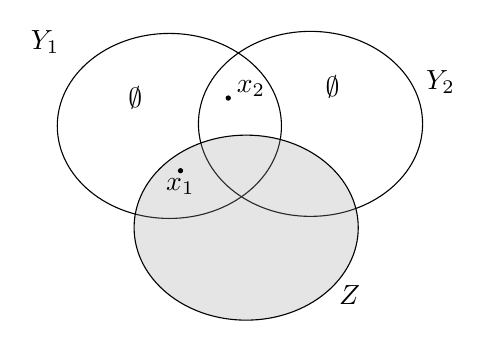
\begin{tikzpicture}[x=0.75pt,y=0.75pt,yscale=-1,xscale=1]
			%uncomment if require: \path (0,300); %set diagram left start at 0, and has height of 300

			%Shape: Ellipse [id:dp4986066503370681] 
			\draw   (186,119.57) .. controls (186,94.96) and (210.18,75) .. (240,75) .. controls (269.82,75) and (294,94.96) .. (294,119.57) .. controls (294,144.19) and (269.82,164.15) .. (240,164.15) .. controls (210.18,164.15) and (186,144.19) .. (186,119.57) -- cycle ;
			%Shape: Ellipse [id:dp843936435141502] 
			\draw   (254,118.57) .. controls (254,93.96) and (278.18,74) .. (308,74) .. controls (337.82,74) and (362,93.96) .. (362,118.57) .. controls (362,143.19) and (337.82,163.15) .. (308,163.15) .. controls (278.18,163.15) and (254,143.19) .. (254,118.57) -- cycle ;
			%Shape: Ellipse [id:dp9951733970596428] 
			\draw  [fill={rgb, 255:red, 155; green, 155; blue, 155 }  ,fill opacity=0.26 ] (223,168.57) .. controls (223,143.96) and (247.18,124) .. (277,124) .. controls (306.82,124) and (331,143.96) .. (331,168.57) .. controls (331,193.19) and (306.82,213.15) .. (277,213.15) .. controls (247.18,213.15) and (223,193.19) .. (223,168.57) -- cycle ;
			%Shape: Circle [id:dp10790237532892788] 
			\draw  [fill={rgb, 255:red, 0; green, 0; blue, 0 }  ,fill opacity=1 ] (267.38,106.14) .. controls (267.38,105.59) and (267.83,105.15) .. (268.37,105.15) .. controls (268.92,105.15) and (269.36,105.59) .. (269.36,106.14) .. controls (269.36,106.68) and (268.92,107.13) .. (268.37,107.13) .. controls (267.83,107.13) and (267.38,106.68) .. (267.38,106.14) -- cycle ;
			%Shape: Circle [id:dp38669899440893385] 
			\draw  [fill={rgb, 255:red, 0; green, 0; blue, 0 }  ,fill opacity=1 ] (244.38,141.14) .. controls (244.38,140.59) and (244.83,140.15) .. (245.37,140.15) .. controls (245.92,140.15) and (246.36,140.59) .. (246.36,141.14) .. controls (246.36,141.68) and (245.92,142.13) .. (245.37,142.13) .. controls (244.83,142.13) and (244.38,141.68) .. (244.38,141.14) -- cycle ;

			% Text Node
			\draw (172,72.5) node [anchor=north west][inner sep=0.75pt]    {$Y_{1}$};
			% Text Node
			\draw (362.5,91.5) node [anchor=north west][inner sep=0.75pt]    {$Y_{2}$};
			% Text Node
			\draw (219,99.5) node [anchor=north west][inner sep=0.75pt]    {$\emptyset $};
			% Text Node
			\draw (314,94) node [anchor=north west][inner sep=0.75pt]    {$\emptyset $};
			% Text Node
			\draw (237.2,143.76) node [anchor=north west][inner sep=0.75pt]    {$x_{1}$};
			% Text Node
			\draw (271.2,96.36) node [anchor=north west][inner sep=0.75pt]    {$x_{2}$};
			% Text Node
			\draw (320.48,195.16) node [anchor=north west][inner sep=0.75pt]    {$Z$};


		\end{tikzpicture}
		\caption{}\label{fig:完美集合族}
	\end{figure}

	因为 $Z$ 为元素最少的非空集合, 且 $Y_{2}$ 不为空集,所以, $|Z| \leqslant\left|Y_{2}\right|$.

	又 $Z \not \subset Y_{2}\left(\right.$ 因 $\left.x_{1} \in Z \backslash Y_{2}\right)$, 可推断 $Y_{2} \backslash Z$ 不为空集.

	因此, 存在元素 $x_{2} \in Y_{2} \backslash Z=Y_{1} \backslash Z$.

	故 $x_{1} \in Z \backslash Y_{2}, x_{2} \in Y_{2} \backslash Z,\left\{x_{1}, x_{2}\right\} \subseteq Y_{1}$.

	当 $X_{1}=Z, X_{2}=Y_{2}, X_{3}=Y_{1}$ 时,这与集合族 $\mathscr{F}$ 是完美的矛盾.

	定义 $\mathscr{F}^{\prime}$ 是 $U \backslash Z$ 的子集构成的集合族 $\mathscr{F}^{\prime}=\{Y \backslash Z \mid Y \in \mathscr{F}, Y \neq \varnothing\}$. 显然,集合族 $\mathscr{F}^{\prime}$ 是一个由更小的子集构成的完美的集合族.

	故由归纳假设, 有 $\left|\mathscr{F}^{\prime}\right| \leqslant|U \backslash Z|+1$.

	此外,由前知集合 $Y \backslash Z$ 是与 $Y \in \mathscr{F}$ 且 $Y \neq \varnothing$ 不同的.

	因此, $|\mathscr{F}| \leqslant\left|\mathscr{F}^{\prime}\right|+1$ ( +1 是因为集合族 $\mathscr{F}$ 中有可能含有空集).

	故 $|\mathscr{F}| \leqslant\left|\mathscr{F}^{\prime}\right|+1 \leqslant|U \backslash Z|+1+1 \leqslant|U|-1+1+1=|U|+1$.
\end{proof}

\begin{example}
	设 $A_{1}, A_{2}, \cdots, A_{n}$ 为有限集合 $X$ 的 $n$ 个非空子集,且对任意正整数 $i 、 j(1 \leqslant i \leqslant j \leqslant n), A_{i} \cap A_{j}$ 不为单元集. 证明: 可将集合 $X$ 的元素分成两类,使每个子集 $A_{i}(i=1,2, \cdots, n)$ 的元素不全在同一类中.
\end{example}

\begin{proof}
	因为每个子集 $A_{i}(i=1,2, \cdots, n)$ 非空,且由条件知 $A_{i}=A_{i} \cap$ $A_{i}$ 不为单元集,所以,集合 $A_{i}$ 至少含两个元素.

	在集合 $X$ 的某种分类下,若 $A_{i}$ 的元素只出现在一类中,则称 $A_{i}$ 为“单类集”;若 $A_{i}$ 的元素出现在两类中,则称 $A_{i}$ 为“双类集”.

	记 $t$ 为 $A_{i}(i=1,2, \cdots, n)$ 中双类集的数目, 若 $t$ 能取到 $n$, 则命题得证.

	因为 $A_{1}$ 至少含两个元素,所以,先将集合 $X$ 的元素分成两类,且使 $A_{1}$ 为双类集. 此时, $t \geqslant 1$.

	下面证明:对使 $t<n$ 的任意一种分类, 经适当调整必可使 $t$ 的值增加.

	设集合 $X$ 中 $x_{1}, x_{2}, \cdots, x_{r}$ 在第一类 $, x_{r+1}, x_{r+2}, \cdots, x_{m}$ 在第二类. 不妨设此时 $A_{1}, A_{2}, \cdots, A_{t}$ 为双类集, $A_{t+1}, A_{t+2}, \cdots, A_{n}$ 为单类集, 且 $A_{t+1}=$ $\left\{x_{1}, x_{2}, \cdots, x_{s}\right\}$, 其中, $A_{t+1}$ 至少含两个元素. 故 $2 \leqslant s \leqslant r$, 这表明,第一类元素不少于两个.

	现将集合 $X$ 中的元素 $x_{1}$ 调到第二类,其余元素类别不变. 此时,集合 $X$仍有两类元素,而 $A_{t+1}$ 变为双类集.

	若 $A_{i}(1 \leqslant i \leqslant t)$ 不含元素 $x_{1}$, 则 $A_{i}$ 仍为双类集; 若 $A_{i}(1 \leqslant i \leqslant t)$ 含元素 $x_{1}$, 则根据条件, $A_{i}$ 与 $A_{t+1}$ 必有除 $x_{1}$ 之外另一公共元素 $x_{j}(2 \leqslant j \leqslant s)$, 故 $x_{1}$调到第二类后, $A_{i}$ 中仍有第一类元素,即 $A_{i}$ 仍为双类集.

	综上, 调整之后至少 $A_{1}, A_{2}, \cdots, A_{t+1}$ 为双类集.

	因此,双类集数目不小于 $t+1$.

	从而, 经有限次这样的调整后必有 $t=n$.
\end{proof}
最后,我们来看一个集合族的例子.

\begin{example}
	给定正整数 $k \geqslant 2$, 请构造一个集合簇 $\mathscr{A}$, 它包含无限多个由正整数构成的集合, 满足以下性质:

	(1) 集合族 $\mathscr{A}$ 中任意 $k$ 个集合的交集为一个单元素集合;

	(2) 集合族 $\mathscr{A}$ 中任意 $k+1$ 个集合的交集为空集.
\end{example}
\begin{solution}
	将正整数集合中任意 $k$ 个数构成的集合无重复无遗漏地排成一排,记这些集合依次为 $S_{1}, S_{2}, \cdots$. 对每个正整数 $m$, 取 $A_{m}=\left\{n \mid m \in S_{n}\right\}$, 集合族 $\mathscr{A}$ 由 $A_{1}, A_{2}, \cdots$ 构成.

	接下来证明集合簇 $\mathscr{A}$ 符合题意.

	首先证明:集合簇 $\mathscr{A}$ 确为一个无限集.

	对于不同的两个正整数 $m 、 m^{\prime}$, 由构造法则, 知存在不同的正整数 $n 、 n^{\prime}$,使得 $m \in S_{n}, m \notin S_{n^{\prime}}$, 但 $m^{\prime} \in S_{n^{\prime}}, m^{\prime} \notin S_{n}$.

	故 $n \in A_{m} \backslash A_{m^{\prime}}, n^{\prime} \in A_{m^{\prime}} \backslash A_{m}$. 从而, $A_{m} \neq A_{m^{\prime}}$.

	其次证明:子集簇  $\mathscr{A}$ 满足性质(1).

	若 $m_{1}, m_{2}, \cdots, m_{k}$ 为不同的正整数,则
	$$
		A_{m_{1}} \cap A_{m_{2}} \cap \cdots \cap A_{m_{k}}=\{i\}
	$$
	其中, $i$ 为集合 $\left\{m_{1}, m_{2}, \cdots, m_{k}\right\}$ 在排列 $S_{1}, S_{2}, \cdots$ 中所在集合的下标.

	最后证明:子集簇 $\mathscr{A}$ 满足性质(2).

	若 $m_{1}, m_{2}, \cdots, m_{k+1}$ 为不同的正整数, 则 $\left\{m_{1}, m_{2}, \cdots, m_{k}\right\} 、\left\{m_{2}, \cdots\right.$, $\left.m_{k}, m_{k+1}\right\}$ 在排列 $S_{1}, S_{2}, \cdots$ 中处于不同位置.

	故 $A_{m_{1}} \cap A_{m_{2}} \cap \cdots \cap A_{m_{k}} \cap A_{m_{k+1}}=\varnothing$.
\end{solution}

\section{集合的性质}
很多集合问题实际上是研究集合的性质的问题. 由集合的概括原则, 我们知道集合 $\{x \mid P(x)\}$ 是由满足性质 $P$ 的元素组成的, 因此除了研究一般集合的性质外, 我们更多地是研究具体的集合所满足的性质 $P$ 的等价形式或推论, 如对特定整数的集合、有理数的集合等的研究.

在这里, 我们无意于也无此必要介绍太多集合论的知识, 利用中学已有的集合知识和解题中体悟的逻辑方法, 我们就能理解本书中的全部内容.

\subsection{集合的整体性质}
已知集合 $S=\{x \mid P(x)\}$. 如果由性质 $P$ 能推出 $S$ 中每个元素都满足的性质 $P^{\prime}$, 那么 $P^{\prime}$ 就是 $P$ 的一个必要条件. 设 $S^{\prime}=\left\{x \mid P^{\prime}(x)\right\}$, 显然有 $S \subseteq S^{\prime}$.
\begin{example}
	已知数集 $M$ 至少有 3 个元素, 且对 $M$ 中任何两个不同的元素 $a$ 、 $b$, 数 $a^{2}+b \sqrt{2}$ 都是有理数, 证明: 对于 $M$ 中任何数 $a$, 数 $a \sqrt{2}$ 都是有理数.
\end{example}
\begin{analysis}
	设 $a, b \in M$ 且 $a \neq b$, 则 $a^{2}+b \sqrt{2} \in \mathbb{Q}, b^{2}+a \sqrt{2} \in \mathbb{Q}$. 于是有 $a^{2}+$ $b \sqrt{2}-\left(b^{2}+a \sqrt{2}\right)=\frac{1}{2}(a \sqrt{2}-b \sqrt{2})(a \sqrt{2}+b \sqrt{2}-2) \in \mathbb{Q}$. 若能证明 $a \sqrt{2}-$ $b \sqrt{2} \in \mathbb{Q}$ 或 $a \sqrt{2}+b \sqrt{2} \in \mathbb{Q}$, 则问题迎刃而解. 但已给条件似乎不够用! 不过另设 $c \in M, c \neq a, c \neq b$, 则 $c^{2}+a \sqrt{2} \in \mathbb{Q}, c^{2}+b \sqrt{2} \in \mathbb{Q}$, 便得到
	$$
		c^{2}+a \sqrt{2}-\left(c^{2}+b \sqrt{2}\right)=a \sqrt{2}-b \sqrt{2} \in \mathbb{Q}
	$$
\end{analysis}
\begin{proof}
	任取 $a, b, c \in M$, 且 $a 、 b 、 c$ 互不相等, 则 $a^{2}+b \sqrt{2}, b^{2}+a \sqrt{2}, c^{2}$ $+a \sqrt{2}, c^{2}+b \sqrt{2} \in \mathbb{Q}$. 因此
	$$
		\begin{aligned}
			  & a^{2}+b \sqrt{2}-\left(b^{2}+a \sqrt{2}\right)=(a-b)(a+b-\sqrt{2})         \\
			= & \frac{1}{2}(a \sqrt{2}-b \sqrt{2})(a \sqrt{2}+b \sqrt{2}-2) \in \mathbb{Q}
		\end{aligned}
	$$

	$$
		c^{2}+a \sqrt{2}-\left(c^{2}+b \sqrt{2}\right)=(a \sqrt{2}-b \sqrt{2}) \in \mathbb{Q}
	$$
	从而 $a \sqrt{2}+b \sqrt{2}-2 \in \mathbb{Q}$, 所以 $a \sqrt{2}+b \sqrt{2} \in \mathbb{Q}$.

	所以

	$$
		a \sqrt{2}=\frac{1}{2}(a \sqrt{2}+b \sqrt{2}+a \sqrt{2}-b \sqrt{2}) \in \mathbb{Q}
	$$
\end{proof}

\begin{example}
	在平面上给定无穷多个点, 已知它们之间的距离都是整数, 求证这些点都在一条直线上.
\end{example}
\begin{analysis}
	“无穷”和“整数”是两个关键词, 去其一, 则结论不成立. 下面我们就是利用这两点“制造”矛盾来反证结论成立.
\end{analysis}
\begin{proof}
	若不然, 则存在三点 $A 、 B 、 C$ 使三点不共线且 $A B=r$ 和 $A C=s$都是整数. 设点 $P$ 是任一给定点, 则由三角不等式有
	$$
		|P A-P B| \leqslant A B=r
	$$
	即 $|P A-P B|$ 是整数 $0,1,2, \cdots, r$ 中之一. 因此,点 $P$ 或位于直线
	$$
		\begin{aligned}
			 & H_{0}=\text { 直线 } A B \text { 的垂直平分线, } \\
			 & H_{r}=\text { 直线 } A B
		\end{aligned}
	$$
	之一上,或落在双曲线
	$$
		H_{i}=\{X|| X A-X B \mid=i\}, i=1,2, \cdots, r-1
	$$
	之一上. 同理, 点 $P$ 又或者位于直线
	$$
		\begin{aligned}
			 & K_{0}=\text { 线段 } A C \text { 的垂直平分线, } \\
			 & K_{s}=\text { 直线 } A C
		\end{aligned}
	$$
	之一上,或者落在双曲线
	$$
		K_{j}=\{X|| X A-X C \mid=j\}, j=1,2, \cdots, s-1
	$$
	之一上. 由此可知, 任一给定点必落在集合
	\begin{equation*}
		H_{i} \cap K_{j}, i=0,1, \cdots, r, j=0,1, \cdots, s \tag{1}
	\end{equation*}
	之一上. 由于直线 $A B$ 与 $A C$ 不重合, 所以任一 $H_{i}$ 与任一 $K_{j}$ 都不相同.从而知(1)中每个集合都不多于 4 点,故知集合
	$$
		M=\bigcup_{i, j}\left(H_{i} \cap K_{j}\right)
	$$
	的点数不多于 $4(r+1)(s+1)$, 此与给定点有无穷多个矛盾.
\end{proof}

\begin{example}
	设 $M$ 为一个无限的有理数集, 满足: $M$ 的任意一个 2009 元子集的元素之积为一个整数,且这个整数不能被任何质数的 2009 次幂整除. 证明: $M$的元素均为整数.
\end{example}
\begin{analysis}
	这里的“2009”并不是一个关键的数字, 与上例一样, 我们还是得围绕“无限”做文章.
\end{analysis}
\begin{proof}
	设 $a_{1}, a_{2}, \cdots, a_{2008} \in M$. 记
	$$
		A=a_{1} a_{2} \cdots a_{2008}=\frac{p}{q},(p, q)=1
	$$

	假设 $M$ 中包含了无数多个形如
	$$
		\alpha_{i}=\frac{p_{i}}{q_{i}},\left(p_{i}, q_{i}\right)=1, q_{i}>1
	$$
	的数,且 $\alpha_{i} \neq a_{1}, a_{2}, \cdots, a_{2008}$. 由于
	$$
		\alpha_{i} \cdot A=\alpha_{i} a_{1} a_{2} \cdots a_{2008}=\frac{p_{i}}{q_{i}} \cdot \frac{p}{q}
	$$
	为整数,所以
	$q \mid p$
	由于 $p$ 只有有限个因子, 故有无数个分母为 $q_{i}^{\prime}$ 的既约分数属于 $M$. 这些分数中的任意 2009 个的乘积都不是整数. 这与题设矛盾. 这说明 $M$ 中包含了无限多个整数,记这些整数的集合为 $M^{\prime}$.

	假设有 $\frac{a}{b} \in M,(a, b)=1, b>1$.

	设 $p$ 为 $b$ 的一个质因子. 由于 $\frac{a}{b}$ 与 $M^{\prime}$ 中任意 2008 个整数的乘积为整数,故 $p$ 为 $M^{\prime}$ 中无数多个整数的质因子. 而 $M^{\prime}$ 中任意 2009 个含有因数 $p$ 的数的乘积可被 $p^{2009}$ 整除. 这又与题设矛盾.

	这就证明了 $M$ 的元素均为整数. 而这样的整数集是存在的,如全部质数的集合.
\end{proof}

\begin{example}
	设七元素集合 $A=\left\{a_{1}, a_{2}, \cdots, a_{7}\right\}$ 的元素均为不大于 26 的正整数. 证明: 存在正整数 $t 、 m(1 \leqslant t<m \leqslant 7)$, 使得方程
	$$
		x_{1}+x_{2}+\cdots+x_{t}=x_{t+1}+x_{t+2}+\cdots+x_{m}
	$$
	在集合 $A$ 上有解,且 $x_{1}, x_{2}, \cdots, x_{m}$ 互不相等.
\end{example}
\begin{analysis}
	如能证明集合 $A$ 有两个互不包含的子集的元素和相等, 则求证结论成立.
\end{analysis}
\begin{proof}
	首先证明:在集合 $A$ 的最多含有四个元素的子集中,有两个集合的元素之和是相等的.

	易知,集合 $A$ 的最多含有四个元素的非空子集有 $\mathrm{C}_{7}^{1}+\mathrm{C}_{7}^{2}+\mathrm{C}_{7}^{3}+\mathrm{C}_{7}^{1}=98$ (个). 这些子集的元素之和的最小可能值为 1 , 最大可能值为 $26+25+24+$ $23=98$.

	假设在这些子集中没有两个的元素之和是相等的. 则 $1 \sim 98$ 的每个整数恰分别是上述 98 个子集的元素之和.

	特别地, 98 是子集 $\{23,24,25,26\}$ 的元素之和.

	故 $\{23,24,25,26\} \subset A$.

	所以, $\{23,26\} \subset A$, 且 $\{24,25\} \subset A$.

	而 $\{23,26\}$ 与 $\{24,25\}$ 的元素之和相等. 矛盾.

	设 $B_{1} 、 B_{2}$ 是集合 $A$ 的两个元素之和相等的子集, $B_{1} \cap B_{2}=C$. 则 $B_{1}^{\prime}=$ $B_{1} \backslash C, B^{\prime}{ }_{2}=B_{2} \backslash C$ 也是集合 $A$ 的非空子集.

	设 $\left|B_{1}^{\prime}\right|=t,\left|B_{2}\right|=m-t$. 记 $B_{1}^{\prime}$ 的元素分别为 $x_{1}, x_{2}, \cdots, x_{t}, B_{2}^{\prime}$ 的元素分别为 $x_{t+1}, x_{t+2}, \cdots, x_{m}$, 即得方程的一组解.
\end{proof}

\subsection{集合的局部性质}
设集合 $S=\{x \mid P(x)\}$. 如果条件 $P^{*}$ 是条件 $P$ 的充分条件, 那么集合
$$
	S^{*}=\left\{x \mid P^{*}(x), x \in S\right\}
$$
是集合 $S$ 的子集,即 $S^{*} \subseteq S$. 这里 $P^{*}$ 是集合 $S$ 中部分元素的性质.

我们还可以通过增加 $S$ 的“内涵”的方式来缩小它的“外延”: $S$ 是所有具备性质 $P$ 的元素 $x$ 的集合,增加新的性质 $P^{*}$, 得到集合
$$
	S^{*}=\left\{x \mid P(x) \text { 且 } P^{*}(x), x \in S\right\},
$$

显然 $S^{*}=\left\{x \mid P^{*}(x), x \in S\right\}$, 它是 $S$ 的子集, 即 $S^{*} \subseteq S$.

一类典型的问题就是从集合 $S$ 中分离出所有满足性质 $P^{*}$ 的元素, 从而得到所求的 $S^{*}$.

\begin{example}
	设 $A \subset \mathbb{N}^{*}$ 是无限集, $A$ 中每个数 $a$ 是至多 1990 个质数的乘积. 证明: 必有 $A$ 的无限子集 $B$, 使得 $B$ 中任何两个不同数的最大公因数都相同.
\end{example}
\begin{analysis}
	如果 $A$ 中含有无限多个两两互质的整数, 则结论显然成立. 否则,存在质数 $p_{1}$ 为 $A$ 的无限多个数的因数, 故 $A_{1}=\left\{\frac{a}{p_{1}} \left\lvert\, \frac{a}{p_{1}} \in \mathbb{Z}\right., a \in A\right\}$ 为无限集. 若 $A_{1}$ 中含有无限多个两两互质的整数,则结论亦成立. 否则, 继续上面的步骤.
\end{analysis}
\begin{proof}
	如果 $A$ 中含有无限多个两两互质的正整数, 将它们全部选出作成子集 $B$, 则结论成立.

	若存在质数 $p_{1}$ 为 $A$ 中无限多个数的因数, 则集合
	$$
		A_{1}=\left\{\frac{a}{p_{1}} \left\lvert\, \frac{a}{p_{1}} \in \mathbb{Z}\right., a \in A\right\}
	$$
	为无限集. 依此类推 (用 $A_{1}$ 代替 $A$ ). 由于 $A$ 中每个数的质因数个数 $\leqslant 1990$,所以必有无限集
	$$
		A_{k}=\left\{\frac{a}{p_{1} p_{2} \cdots p_{k}} \left\lvert\, \frac{a}{p_{1} p_{2} \cdots p_{k}} \in \mathbb{Z}\right., \frac{a}{p_{1} p_{2} \cdots p_{k-1}} \in A_{k-1}\right\},
	$$

	每个质数 $p_{i}$ 都仅是 $A_{k}$ 中有限多个数的因数.

	任取 $a_{1} \in A_{k}$. 在取定 $a_{1}, a_{2}, \cdots, a_{n}$ 两两互质后, 由于每个质数都仅是 $A_{k}$ 中有限多个数的因数, 在 $A_{k}$ 中存在 $a_{n+1}$, 它与 $a_{1}, a_{2}, \cdots, a_{n}$ 均互质. 这样就得到 $A_{k}$ 的一个无穷子集 $B_{k}, B_{k}$ 中的元素两两互质.

	将 $B_{k}$ 中每个元素乘以 $p_{1} p_{2} \cdots p_{k}$, 得到 $A$ 的无穷子集, 其中每两个数的最大公因数均为 $p_{1} p_{2} \cdots p_{k}$.
\end{proof}

\begin{example}
	记 $\mathbb{Q}$ 为有理数集合, $\mathbb{Q}$ 的非空子集 $S$ 具有以下性质:

	(1) $0 \notin S$;

	(2) 若 $s_{1} \in S, s_{2} \in S$, 则 $\frac{s_{1}}{s_{2}} \in S$;

	(3) 存在一非零有理数 $q, q \notin S$, 且每一个不在 $S$ 中的非零有理数都可写成 $q s$ 的形式, 其中 $s \in S$.

	证明: 若 $x \in S$, 则存在 $y, z \in S$, 使 $x=y+z$.
\end{example}
\begin{analysis}
	设 $\alpha, \beta \in \mathbb{Q}$, 且 $\alpha+\beta=1$, 则
	$$
		x=x(\alpha+\beta)=x \alpha+x \beta
	$$

	我们希望出现: $x \alpha \in S$ 且 $x \beta \in S$. 由 (3) 似乎应该有 $\alpha, \beta \in S$. 于是我们要解决两个问题: (1) 怎样的 $\alpha, \beta$ 必定属于 $S$; (2) 如 $x_{1} \in S, x_{2} \in S$, 则 $x_{1} x_{2} \in S$.
\end{analysis}
\begin{proof}
	假设 $s \in S$. 令 $s_{1}=s_{2} \in S$, 则 $\frac{s_{1}}{s_{2}}=1 \in S$. 令 $s_{1}=1, s_{2}=s$, 则 $\frac{1}{s} \in S$.

	若 $t \in S$, 令 $s_{1}=t, s_{2}=\frac{1}{s}$, 则 $\frac{s_{1}}{s_{2}}=\frac{t}{\frac{1}{s}}=s t \in S$ (这样 $s$ 就是乘法意义下的解).\\
	假设 $u$ 是一个非零有理数, 若 $u \notin S$, 则 $u=q s$, 其中 $s \in S$, 于是我们有 $u^{2}=q^{2} s^{2}$.

	若 $q^{2} \notin S$, 则可设 $q^{2}=q t(t \in S)$, 则 $q=t \in S$, 矛盾. 所以 $q^{2} \in S$, $u^{2} \in S$.

	假如 $x \in S$, 则由 $\left(\frac{3}{5}\right)^{2} 、\left(\frac{4}{5}\right)^{2}$ 为平方数可知,
	$$
		x\left(\frac{3}{5}\right)^{2} \in S, x\left(\frac{4}{5}\right)^{2} \in S
	$$
	又 $x=x\left(\frac{3}{5}\right)^{2}+x\left(\frac{4}{5}\right)^{2}$, 取 $y=x\left(\frac{3}{5}\right)^{2}, z=x\left(\frac{4}{5}\right)^{2}$, 则命题得证.
\end{proof}

\begin{example}
	平面上整点的集合 $M=\{(x, y) \mid x, y \in \mathbb{Z}$, 且 $1 \leqslant x \leqslant 12,1 \leqslant$ $y \leqslant 13\}$. 证明: 不少于 49 个点的 $M$ 的每一个子集,必包含一个矩形的 4 个顶点,且此矩形的边平行于坐标轴.
\end{example}

\begin{analysis}
	设 $S$ 为 $M$ 的任一个 49 元子集. 其中纵坐标相同的点的横坐标的集合为:
	$$
		X_{i}=\{x \mid(x, i) \in S\}, i=1,2, \cdots, 13
	$$
	若存在关于整点横坐标的二元集 $(r, s)$ 同时是 $X_{i} 、 X_{j}(i \neq j)$ 的子集,则原题得证.
\end{analysis}
\begin{proof}
	设 $S$ 为 $M$ 的任一个 49 元子集. 令
	$$
		X_{i}=\{x \mid(x, i) \in S\}, i=1,2, \cdots, 13
	$$
	则 $\left|X_{i}\right|=x_{i}, \sum_{i=1}^{13} x_{i}=49,0 \leqslant x_{i} \leqslant 12$. 记
	$$
		P_{i}=\{\{r, s\} \mid r \neq s,(r, i),(s, i) \in S\}, i=1,2, \cdots, 13
	$$
	显然, 全体 $P_{i}$ 中只有 $\mathrm{C}_{12}^{2}=66$ (种) 不同的二元集.

	又 $\sum_{i=1}^{13}\left|P_{i}\right|=\sum_{i=1}^{13} \mathrm{C}_{x_{i}}^{2}$, 考虑其最小值.

	利用局部调整: 当 $x_{1}+x_{2}=c$ 时,
	$$
		\mathrm{C}_{x_{1}}^{2}+\mathrm{C}_{x_{2}}^{2}=\frac{c^{2}-c}{2}-x_{1} x_{2} \geqslant \frac{c^{2}-c}{2}-\frac{c^{2}}{4},
	$$

	$x_{1}=\left[\frac{c}{2}\right], x_{2}=c-\left[\frac{c}{2}\right]$ 时, $\mathrm{C}_{x_{1}}^{2}+\mathrm{C}_{x_{2}}^{2}$ 取得最小值. 由此知, $\sum_{i=1}^{13} \mathrm{C}_{x_{i}}^{2}$ 取得最小值必须是将 $49=\sum_{i=1}^{13} x_{i}$ 尽可能地平均到 $\left\{x_{i}\right\}$ 中, 即 $\left\{x_{i}\right\}$ 中有 $j$ 个 $\left[\frac{49}{13}\right]=3$,\\
	$(13-j)$ 个 $\left[\frac{49}{13}\right]+1=4$, 从而得 $j=3$.
	所以
	$$
		\left(\sum_{i=1}^{13} \mathrm{C}_{x_{i}}^{2}\right)_{\min }=3 \mathrm{C}_{3}^{2}+10 \mathrm{C}_{4}^{2}=69
	$$
	从而, 有
	$$
		\sum_{i=1}^{13}\left|P_{i}\right|=\sum_{i=1}^{13} \mathrm{C}_{x_{i}}^{2} \geqslant 69>66
	$$
	由此推知存在 $i \neq j$, 使得 $(r, s) \in P_{i},(r, s) \in P_{j}$.故有 $(r, i),(s, i),(r, j),(s, j) \in S$, 结论成立.
\end{proof}

\subsection	{集合间的相关性质}
\begin{example}
	记 $A$ 为含有 $t\left(t \in \mathbb{R}_{+}\right)$的实数集, 使得存在一个实数集 $B$ (与 $A$ 有关), $|B| \geqslant 4, A B=\{a b \mid a \in A, b \in B\}$ 的元素构成一个有限长等差数列.求集合 $A$ 所有可能的情形.
\end{example}
\begin{analysis}
	若 $|A| \geqslant 2$, 设 $x, x^{\prime} \in A\left(x \neq x^{\prime}\right), y, y^{\prime} \in B\left(y \neq y^{\prime}\right)$, 数列公差为 $d$, 则 $x y-x y^{\prime}=n d(n \in \mathbb{Z})$, 即 $x=n \cdot \frac{d}{y-y}$. 这说明将集合 $A$ 中的元素同时乘以 $\frac{y-y^{\prime}}{d}$, 即可将集合 $A$ 转化为一个整数集来讨论.
\end{analysis}
\begin{solution}
	所求的集合为 $\{t\} 、\{-t, t\} 、\{0, t\} 、\{-t, 0, t\}$.

	只需取 $B=\{-1,0,1,2\}$ 即可验证.

	下面假设集合 $A 、 B$ 符合题意且 $|A| \geqslant 2$.

	显然, $A 、 B$ 元素个数均必须有限.

	记 $d$ 为集合 $A B$ 中等差数列的公差, 任取 $x, x^{\prime} \in A, x \neq x^{\prime}, y, y^{\prime} \in B$, $y \neq y^{\prime}$.

	由于 $x y 、 x y^{\prime}$ 为等差数列中的项,于是,
	$$
		x y-x y^{\prime}=n d(n \in \mathbb{Z}),
	$$

	则 $x=n \cdot \frac{d}{y-y^{\prime}}$.

	这表明, 集合 $A$ 中的任意元素均为 $\frac{d}{y-y}$ 的整数倍.

	从而, 将集合 $A$ 中每个元素除以 $\frac{d}{y-y}$, 使得 $A$ 中每个元素均可化为整数.

	类似地, 对集合 $B$ 中的元素作除以 $\frac{d}{x-x}$ 的处理使得均化为整数.

	接下来, 可将集合 $A$ 中元素除以整体的公约数, 使得整体互质, 对集合 $B$ 也作类似处理.

	记集合 $A$ 中绝对值最大的元素为 $a^{\prime}$, 不妨设 $a^{\prime}>0$. 否则, 将所有元素乘以 -1 即可.

	类似地,记集合 $B$ 中绝对值最大的元素为 $b^{\prime}>0$.

	下面证明: $A=\{-1,1\},\{0,1\},\{-1,0,1\}$.

	因为集合 $B$ 中元素整体互质,而
	$$
		d \mid\left(x-x^{\prime}\right) y \quad\left(x, x^{\prime} \in A, x \neq x^{\prime}, y \in B\right)
	$$

	所以, $d \mid\left(x-x^{\prime}\right)$.

	类似地, $d \mid\left(y-y^{\prime}\right)$.

	而 $|B| \geqslant 4$ 故 $b^{\prime}>d$.

	由于 $a^{\prime} b^{\prime}-d \in A B$, 可设 $a^{\prime} b^{\prime}-d=a b(a \in A, b \in B)$.

	而 $a b=a^{\prime} b^{\prime}-d \geqslant b^{\prime}-d>0$,若 $|a| \neq a^{\prime}$, 则
	$$
		a^{\prime} b^{\prime}-d=a b=|a||b| \leqslant\left(a^{\prime}-1\right) b^{\prime}<a^{\prime} b^{\prime}-d
	$$
	矛盾.

	故 $|a|=a^{\prime}, d=a^{\prime} b^{\prime}-|a||b|=\left(b^{\prime}-|b|\right) a^{\prime} \geqslant a^{\prime}$.

	又集合 $A$ 中所有元素模 $d$ 相同,则
	$$
		A=\{-d, 0, d\},\left\{a^{\prime}, a^{\prime}-d\right\}\left(d \geqslant a^{\prime}>\left|a^{\prime}-d\right|\right)
	$$

	对于前一种情形, 有 $A=\{-t, 0, t\}$.

	对于后一种情形, 若为 $\{0, d\}$, 则对应的 $A=\{0, t\}$. 除此以外, 由 $|a|=$ $a^{\prime}>\left|a^{\prime}-d\right|$, 则
	$$
		a=a^{\prime}, d=a^{\prime}\left(b^{\prime}-|b|\right)
	$$

	从而 $a^{\prime} \mid d$, 则 $a^{\prime} \leqslant \frac{d}{2}$.

	若 $d$ 为偶数, 则可取 $\left\{-\frac{d}{2}, \frac{d}{2}\right\}$, 对应的 $A=\{t,-t\}$; 若 $a^{\prime}<\frac{d}{2}$, 则 $\left|a^{\prime}-d\right|>a^{\prime}$, 矛盾.
\end{solution}

\begin{example}
	在一次数学竟赛中,一些同学间是朋友关系,且朋友关系是相互的. 证明: 存在由学生组成的一个子集 $M$, 使得集合 $M$ 中的每名同学在此集合中至多有三位朋友,不属于集合 $M$ 的每名同学在集合 $M$ 中至少有四位朋友.
\end{example}
\begin{proof}
	设 $M_{0}=\varnothing$. 给出如下构造:

	(1) 若学生 $x \in M$, 其在集合 $M$ 中至少有四位朋友, 则将其从集合 $M$ 中移出;

	(2)若学生 $y \notin M$, 其在集合 $M$ 中最多有三位朋友,则将其移人集合 $M$ 中.

	利用如上两种方法, 可构造满足题意的状态.

	对于集合 $M$, 若 $x 、 y$ 为集合 $M$ 中的朋友, 记 $p(M)$ 表示 $(x, y) \in M \times M$的对数. 设
	$$
		f(M)=7|M|-p(M)
	$$
	注意到, $f(M)$ 仅能取到整数, 且不大于 $7|M|$, 初值为 $f\left(M_{0}\right)=0$.

	由(1)对于 $x \in M, x$ 在集合 $M$ 中至少有四位朋友, 知 $(x, y),(y, x) \in$ $M \times M$ 至少有八对. 因此,若从集合 $M$ 中移出 $x$,则 $p(M)$ 至少减少 $8,|M|$ 减少 1 . 此时, $f(M)$ 增加了.

	接下来, 由 (2)对于 $y \notin M, y$ 在集合 $M$ 中最多有三位朋友, 将 $y$ 添人集合 $M$ 中,则 $p(M)$ 至多增加 $6,|M|$ 增加 1 . 此时, $f(M)$ 也增加了.

	操作 $(1)$ 、 (2) 均使 $f(M)$ 增加, 而 $f(M)$ 有上界, 故操作一定会停止, 此时的 $M$ 即为所要的子集.
\end{proof}

\begin{example}
	已知集合 $X=\{1,2, \cdots, 8\}$. 现有 $k$ 种颜色给 $X$ 的三元子集染色,要求任意两个没有公共元素的三元子集有不同颜色. 证明:

	(1) 四种颜色可以完成染色;

	(2) 三种颜色无法完成染色.
\end{example}
\begin{proof}
	(1) 设四种颜色分别为 $1 、 2 、 3 、 4, A$ 为 $X$ 的一个子集, $m_{A}$ 为其中最大元素值.

	规定:给子集 $A$ 染的颜色为 $\max \left\{1, m_{A}-4\right\}$.

	若两个子集 $A 、 B$ 无公共元素, 则至少在 $m_{A} 、 m_{B}$ 中有一个大于或等于 6 .于是, 两个集合不能全染为 1 号色. 相反, 若两个集合均染一种大于 1 的颜色,则 $m_{A}=m_{B}$, 与两集合不存在公共元素矛盾.

	所以,用四种颜色可以完成染色.

	(2) 将自然数 $1,2, \cdots, 8$ 分别标记为一个立方体的八个顶点, 同时, 标出三元集合 $\{a, b, c\}$ 所对应的三角形的重心. 以下将用各个三角形的重心来代替三元集合.

	接下来证明:无法用三种颜色完成染色.

	只考虑立方体表面上的点.

	若两个三元子集在立方体中分别表示两个相对平面的顶点, 则其必无公共元素. 所以, 立方体一个面上的所有点的颜色必与其对面上点的颜色不同.\\
	假设三种颜色能够完成染色任务. 故在一组对面中, 必有一个面中所有点的颜色相同, 也就是说在立方体表面上必有三个面为单染色面, 设为 $F_{1}$ 、 $F_{2} 、 F_{3}$.

	因为三个面中任意两个面都不平行, 所以, 每两个面都有一个公共的边,且三边交于一点. 设这三个面的顶点分别为
	$$
		\{a, b, c, d\},\{a, b, e, f\},\{a, c, e, g\}
	$$

	因为在三个面中, 每两个面都含有一组不共点的三角形, 所以, 三个面的颜色必为三种不同颜色.

	设 $h$ 为点 $a$ 的对顶点. 则以 $\{f, g, h\}$ 为顶点的三角形颜色与以 $\{a, b$, $c\} 、\{a, b, e\} 、\{a, c, e\}$ 为顶点的三角形颜色不同. 而此三个三角形又分别在面 $F_{1} 、 F_{2} 、 F_{3}$ 上. 于是, 需要第四种颜色.

	综上, 三种颜色无法完成染色任务.
\end{proof}


% \section{集合中的最大(小)值}
% \section{集合的分划}
% \section{分类原则}
% \section{极端原理}
% \section{ 容斥原理}
% \section{ 映射方法}